\chapter{第一个人工智能项目}

% 本章将从探讨为什么 Python 是开启初学者导向的人工智能项目的理想选择到介绍第一个人工智能项目一系列过程。首先简要介绍 Python 语言本身,强调其简洁的语法和强大的社区支持,这使得它成为学习编程和机器学习的理想起点。接下来介绍一些项目前置知识,包括 Python 生态系统中的一些常用库,如 Pandas、Matplotlib 等,这些工具能够高效地处理数据、进行可视化,并构建出功能完整的模型。本项目还会深入讲解如何使用这些库来准备数据集、探索数据特征以及展示分析结果,为后续的模型训练做好充分准备。为了使理论与实践相结合,后续将通过一个具体的猫狗识别项目来引导初学者,这个项目不仅涵盖了从数据预处理到模型训练的完整工作流程,还展示了如何利用现有的深度学习框架快速搭建和评估模型。通过动手操作,读者不仅能加深对概念的理解,还能积累宝贵的实践经验,为未来更复杂的项目打下坚实的基础。

人工智能的学习不仅涉及理论的掌握,更注重通过实践将知识转化为解决实际问题的能力。本章围绕“第一个人工智能项目”展开,系统呈现从基础理论到实践应用的完整过程。内容涵盖Python作为人工智能编程语言的优势,以及其在智能系统构建中的关键作用。从数据预处理开始,逐步展示深度学习模型的搭建与优化方法,并对项目的各个环节进行全面解析,包括数据处理、模型设计、训练测试和结果可视化等过程。通过完整的项目实践,充分体现了理论与实践的结合,为后续复杂项目的开发奠定了坚实基础,同时展现了人工智能技术在实际应用中的价值与成效。

\section{人工智能的编程语言Python}

在人工智能技术快速发展的时代,选择合适的编程语言就如同为项目确定了正确的技术方向,这一选择直接影响着项目的开发效率、可扩展性和实际应用效果。Python作为编程语言,其被广泛推荐为开启人工智能之旅的理想选择。Python具有这样的地位,主要归功于其简洁易读的语法、强大的功能以及丰富的工具库。此外,Python自1991年发布以来,以直观的设计理念迅速成长为适应多种需求的全能型语言。特别是在数据科学和机器学习领域,Python凭借NumPy、SciPy、scikit-learn、TensorFlow和PyTorch等库简化了数值计算、数据分析及人工智能模型构建的过程。

Python的强大不仅体现在技术层面,还在于它背后有一个庞大且活跃的社区。这个社区不断贡献开源项目和技术支持,形成了一个丰富多彩的生态系统,对于新手开发者尤其友好。无论是大型科技公司还是初创企业,Python都是推动人工智能研究和产品开发的重要工具。此外,选择Python进行人工智能开发,不仅能享受到高效便捷的编程体验,还能获得来自社区的广泛支持。随着技术的进步,Python及其生态将继续扩展人工智能技术的应用边界,为开发者提供无限可能。

\subsection{Python简介与特点}

\subsubsection{1. 量身定制的编程语言}

Python是一种设计直观、语法简洁的编程语言,其代码风格接近自然语言,减少了复杂符号和语法规则的使用。因为其一致性高的逻辑结构使得学习新概念更加容易,并且提供了详尽的学习资源,能够有效帮助编程初学者快速上手并写出有用的程序。此外,Python支持多种编程范式——无论是面向对象编程(OOP)、过程化编程还是函数式编程,都能很好地适应。这种灵活性如同一把万能钥匙,允许开发者根据个人偏好或具体问题选择最适合的编程方式,从而更高效地解决问题。无论读者喜欢结构化的解决方案还是灵活多变的方法,Python都能满足需求,让编程变得更加得心应手。

\subsubsection{2. 学习曲线与开发效率}

Python作为一种高效的编程语言,特别适合于将初步概念迅速转换为实际的代码和功能。特别是在人工智能领域,Python的速度优势使得开发者可以快速搭建基础框架,导入必要的库,并立即运行程序进行测试。例如,在构建一个简单的图像识别人工智能模型时,Python允许用户在短时间内完成从设计到实现的过程。这种快速迭代的能力对于探索不同算法、优化模型参数至关重要,因为它加速了学习过程,促进了更快的改进。

Python的动态类型系统和强大的交互式开发环境(如Jupyter Notebook),极大地简化了调试和问题解决的过程。这些工具提供了即时反馈机制,使开发者可以在编写代码的同时验证每一行代码的效果。例如,当遇到不确定的逻辑时,可以直接在交互式shell中运行相关代码片段,检查输出是否符合预期。如果结果不理想,可以立即调整代码并再次测试,整个过程高效流畅。此外,Python无需提前声明变量类型,这增加了编程的灵活性,让代码编写和修改更加便捷。

Python不仅自身功能强大,还能够与其他编程语言和技术无缝协作,成为复杂项目中不可或缺的一部分。在人工智能项目中,经常需要整合多种技术,如使用C++编写高性能计算模块,或者结合Java的企业级应用。Python作为一个超级中介,通过其丰富的库和工具集,轻松实现了这些不同组件之间的连接。例如,在开发人脸识别系统时,可能需要利用深度学习框架(如TensorFlow或PyTorch)处理图像数据,同时调用硬件接口或Web API获取实时信息。Python凭借其强大的集成能力,确保各个部分协同工作,共同完成复杂的任务。

% \subsubsection{3. 社区与资源背景}

% 选择 Python 作为编程语言,意味着加入一个全球性的开发者和爱好者社群。无论是在白天遇到问题还是在深夜萌生新的想法,几乎总能在这个活跃的社区中找到帮助和支持。Python 社区以其包容性和友好性著称,为初学者提供了无与伦比的学习环境。如图\ref{fig:Python社区}所示,社区成员乐于分享经验、技巧及最佳实践,促进了知识的快速传播和个人的成长。

% \begin{figure}[H]
%     \centering
%     \includegraphics[width=0.8\linewidth]{image/6/Python社区.png}
%     \caption{Python社区}
%     \label{fig:Python社区}
% \end{figure}

% Python 社区的开放性和协作精神确保了学习过程既轻松又愉快。对于初学者而言,这种支持尤为宝贵。无论学习偏好是通过阅读书籍、观看视频教程还是参与实际项目,Python 社区都能提供丰富的资源来满足多样化的需求。在线平台上的教程、文档、课程和论坛构成了一个全面的支持网络,使得每个学习者都能找到适合自己的学习路径。此外Python 不仅仅是一种编程语言;它是一个不断发展的生态系统,涵盖广泛的库、框架和工具。这个生态系统紧跟技术进步的步伐,确保 Python 始终位于科技前沿。

% 每当某一领域出现突破性成果时,Python 社区都会及时响应,开发出相应的资源和工具。因此,选择 Python 就是选择了持续学习和创新的机会。无论是当前流行的深度学习、数据分析,还是未来可能出现的新技术,Python 都提供了先进且适用的工具。这不仅能够紧跟时代步伐,还能促进在学术和个人发展中的成长与创新。

\subsection{Python在人工智能中的作用}

\subsubsection{1. 连接研究与应用的过程}

无论是研究人员探索新的机器学习算法,还是企业希望快速验证新技术的可行性,Python都提供了必要的工具和支持。同时研究人员可以利用Python编写代码来迅速验证新算法的有效性。例如,一个新提出的机器学习算法可以通过Python实现,并通过实验数据进行测试,以证明其理论上的优势,其拥有如NumPy、SciPy等科学计算库,使得即使是复杂的数学公式也能轻松实现。这不仅加速了科研过程,还确保了结果的准确性和可靠性。

Python在连接学术研究与产业实践之间架起了一座坚实的桥梁,确保每一项有价值的科研成果都能顺利进入市场。这种转化过程通常包括以下几个步骤:使用Python及其丰富的机器学习库(如TensorFlow、PyTorch)进行模型的构建和优化,通过基于Python开发的原型帮助企业快速评估新技术的应用潜力,最后通过Flask、Django等Web框架以及Kubernetes等容器编排工具,Python支持将人工智能模型部署到云端或嵌入式设备中,满足不同场景的需求。

\subsubsection{2. 生态丰富性与层次性}

Python 编程语言及其生态系统提供了一个层次分明且功能完备的工具集,覆盖了从基础数据处理到复杂模型部署的所有关键步骤。该生态系统确保开发者在项目开发的每一个环节都能找到合适的工具和技术支持,其全面的支持体系涵盖了数据准备、模型训练、性能评估以及最终的产品部署。其中各个阶段提供工具不仅强大而且易于使用,初学者可以在友好的环境中轻松入门,而有经验的开发者则可以利用其灵活性迅速迭代算法,找到最适配问题的解决方案。在性能评估阶段,Python 提供的验证和优化工具保证了模型的准确性与可靠性。因此,Python 以其结构严谨且功能全面的特性,连接并强化了人工智能开发的各个阶段,成为众多人工智能领域相关开发者的首选编程语言。这种层次化且全面的支持体系使得 Python 在每个开发阶段都能为用户提供强有力的支持,无论是新手还是专业人士,都能从中受益。

\subsubsection{3. 贯穿人工智能项目全流程}

Python 作为一种强大且灵活的编程语言,在连接学术研究与产业应用方面扮演了至关重要的角色。它不仅促进了新技术从实验室到市场的快速转化,还在整个人工智能项目生命周期中提供了强有力的支持,确保每个阶段的任务都能高效完成。Python 的生态系统专门为数据处理、模型训练、性能评估以及结果展示等各个阶段准备了大量的简单易用工具,简化了操作流程,使得即使没有丰富经验的用户也能顺利开展开发工作。接下来将详细探讨 Python 生态系统中的具体工具和技术,它们如何在整个人工智能项目生命周期的不同阶段——从初步的数据探索到最终的产品部署——为用户提供全面而有力的支持。

\begin{itemize}
\item \textbf{数据准备}

在启动任何人工智能项目之前,数据的质量和完整性如同建筑中砖块的质量一样至关重要。高质量的数据是构建有效模型的基础,而 Python 在此过程中扮演了“砖瓦匠”的关键角色,通过其强大的数据处理能力,确保数据的收集、清洗和预处理达到高标准,为后续分析和建模工作奠定坚实基础。面对杂乱无章的数据集——其中可能包含缺失值、错误信息或格式不一致的问题——Python 提供了一系列工具和库,如 Pandas 和 NumPy,这些工具能够高效地清理和整理数据。简单来说,开发者可以利用 Pandas 进行数据框操作,轻松处理缺失数据、剔除异常值,并进行数据转换;同时,NumPy 提供了高效的数值计算功能,支持大规模数据的操作和分析。通过这些库的帮助,原本复杂的数据准备工作变得更为系统化和自动化,大大提高了数据准备工作的效率与准确性。



\item \textbf{模型验证与参数优化}

在选定算法并完成模型训练之后,确保模型的可靠性成为下一关键步骤。此过程类似于对新建筑进行结构安全评估,旨在确认模型在各种条件下都能提供稳定且准确的预测结果。Python及其丰富的库为这一阶段提供了强有力的支持。为了保证模型的性能,可以采用诸如交叉验证(Cross-Validation)等统计方法来评估模型的一致性和泛化能力:通过将数据集分割成多个子集,并轮流将每个子集作为验证集,其他部分作为训练集,进而更全面地评估模型的表现。如果在验证过程中发现模型结果波动较大或误差较高,可以通过调整模型参数来改善性能。

PyTorch及其生态系统为模型的参数优化提供了丰富的工具和接口,支持研究人员和实践者实现高效直观的调参过程。例如,通过结合使用PyTorch Lightning或Catalyst等高级框架,可以简化训练循环的编写,并集成网格搜索(Grid Search)和随机搜索(Random Search)等传统参数优化策略,以系统化的方式探索超参数空间,从而找到一组最优参数组合来提升模型性能。

\item \textbf{结果展示}

在成功构建并优化模型之后,如何有效地传达分析结果便成为至关重要的环节。此阶段的目标是将复杂的数据科学成果转化为直观易懂的信息,以便不同背景的受众能够理解并利用这些信息进行决策。Python及其相关库在此过程中扮演了关键角色,提供了多种可视化和报告生成工具,以及模型部署的支持。对于结果展示而言,Python拥有强大的数据可视化库,如Matplotlib、Seaborn等可以将模型的预测输出转换为图形化表示,使得技术内外的人员都能快速理解数据背后的意义。此外,通过使用Jupyter Notebook或类似平台,可以创建交互式文档,结合代码、文本、图表和多媒体元素,提供一个动态的展示环境。

\end{itemize}

本小节详细介绍了Python在人工智能项目不同阶段所提供的工具支持,从数据处理到结果展示,各环节均具备便捷易用的解决方案,适用于不同层次的开发需求。接下来的内容将通过前置知识的讲解,为项目的构建做好准备。通过对关键概念和工具的解析,为后续的应用场景和实例提供必要的理论基础,确保项目原型的开发过程更加清晰、有条理。通过这些实践环节,全面展示了Python在人工智能开发中的优势,不仅涵盖了理论讲解,还强化了实际操作能力,为项目开发奠定了扎实的基础。同时,展示了Python强大的工具链和友好的开发环境,使其在人工智能领域具备良好的应用前景。这些实践经验无论是在进一步研究中,还是在实际工作中,都将为后续的技术探索提供重要支持。

\section{前置知识学习}

在开始第一个深度学习项目之前,熟悉相关模块的基本功能与用法是关键。本小节将详细介绍几个核心工具,包括Pandas用于数据管理,Matplotlib和Seaborn用于数据可视化,以及PyTorch作为深度学习框架的核心工具等。这些内容将为后续项目学习提供必要的背景知识,同时奠定进一步探索机器学习领域的基础。

\subsection{Python相关}

\subsubsection{1.多种方式导入模块}

在Python编程中,导入包(或模块)是使用其他人编写的代码来扩展自己程序功能的重要方式。通过导入包,可以利用现成的函数、类和变量,而无需从头开始编写所有代码。这不仅提高了开发效率,还促进了代码的复用性和可维护性。本小节将详细介绍如何在Python中导入包,并解释几种常见的导入方式及其应用场景。

\begin{itemize}
\item \textbf{使用import关键字}

最常用的方式是使用 import 关键字来导入整个包或模块。这样做的好处是可以明确地知道所使用的函数或类来源于哪个包,有助于提高代码的可读性和清晰度。接下来的代码段介绍使用import导入整个包(见程序清单~\ref{import关键字})。

\begin{lstlisting}[language={python},label={import关键字},caption={import关键字}, basicstyle=\footnotesize\ttfamily, breaklines=true, numbers=left, frame=single]
# 导入整个包
# math 模块提供对数学运算的支持,例如三角函数、对数、指数函数等
import math

# 使用包中的函数
print(math.sqrt(16))  # sqrt()函数计算16的平方根,输出: 4.0
\end{lstlisting}

\item \textbf{使用 from ... import ... 语句}

有时只需在代码段中使用包的某些特定函数或类,这时可以使用 from ... import ... 语句来有选择地导入。这种方式可以使代码更简洁,因为可以直接调用导入的对象而不必每次都指定包名。接下来的代码段介绍使用 from ... import ... 导入整个包(见程序清单~\ref{from..import..})。

\begin{lstlisting}[language={python},label={from..import..},caption={from..import..}, basicstyle=\footnotesize\ttfamily, breaklines=true, numbers=left, frame=single]
#导入单个对象
from math import sqrt

# 直接使用导入的函数
print(sqrt(16))  # sqrt函数计算16的平方根,输出: 4.0

\end{lstlisting}

\item \textbf{使用 as 关键字简化名称}

当包名或对象名较长时,可以通过 as 关键字为它们创建一个简短的别名。这不仅能够使代码更加简洁,还可以避免命名冲突。接下来的代码段介绍使用 import 导入包并重命名(见程序清单~\ref{as 关键字})。
\begin{lstlisting}[language={python},label={as 关键字},caption={as 关键字}, basicstyle=\footnotesize\ttfamily, breaklines=true, numbers=left, frame=single,keepspaces=true,showstringspaces=false]
#导入包并重命名
import numpy as np

# 使用别名调用包中的函数
array = np.array([1, 2, 3])
print(array.mean())  # mean()计算array数组的平均值,输出: 2.0

\end{lstlisting}
\end{itemize}

\subsubsection{2.数据结构介绍}

在编程中,数据结构是用来组织、管理和存储数据的方式,进而高效地访问和修改数据。良好的数据结构选择不仅能够简化代码编写,还能显著提升程序的性能和可维护性。Python 作为一种高级编程语言,内置了多种强大的数据结构,包括列表(List)、字典(Dictionary)、元组(Tuple)和集合(Set)。这些数据结构各自具有独特的特性和应用场景,为开发者提供了灵活的数据处理工具。

\begin{itemize}
\item \textbf{字典}

在Python中,字典是一种用于存储数据值的集合,采用键值对的形式。字典的定义强调了其无序性、可变性和不允许重复键的特性。字典通常使用花括号 {} 来创建,键必须是唯一的并且通常是不可变类型(如字符串、数字或元组),而值则可以是任何数据类型,包括其他字典、列表等,每个键与一个值相关联。因此字典非常适合用于查找表或映射关系的表示。

\item \textbf{列表}

在Python中,列表是一种内置的数据结构,用于存储多个项目。同时列表是一个可变的序列,可以包含不同类型的元素,包括数字、字符串和其他对象,可以通过方括号 [] 来创建,元素之间用逗号分隔。

\item \textbf{元组}

在Python中,元组是一种内置的数据类型,用于存储有序的集合。通常使用括号 () 来创建,元素之间用逗号分隔。元组的一个重要特性是不可变性,这意味着一旦创建,元组中的元素不能被修改。因此,元组在需要保护数据不被意外修改的情况下非常有用。此外,元组的元素是有序的,这意味着每个元素都有一个固定的位置,可以通过索引访问,索引从0开始。
\end{itemize}


\subsection{数据预处理}

\subsubsection{1.Numpy}

Numpy(Numerical Python)是Python中广泛使用的科学计算库,提供了多维数组对象(ndarray)以及对这些数组进行操作的各种函数,可以直接作用于整个数组,无需循环遍历每个元素,大大提高了计算效率,常见的操作包括加减乘除、指数、对数、三角函数等,还有统计函数如平均值、方差、标准差等。它不仅支持大规模数值运算,还具备高效的内存管理机制,是数据处理和分析不可或缺的工具。接下来的代码段涵盖如何利用Numpy创建多维数组、执行基本运算以及对多维数组进行简单操作(见程序清单~\ref{Numpy简单操作1}以及程序清单~\ref{Numpy简单操作2})。

\begin{lstlisting}[language={python},label={Numpy简单操作1},caption={Numpy简单操作1}, basicstyle=\footnotesize\ttfamily, breaklines=true, numbers=left, frame=single,keepspaces=true,showstringspaces=false]
# 引入 numpy 库
import numpy as np

# 创建一个一维数组
simple_array = np.array([1, 2, 3, 4, 5])
# 打印创建的数组
print("一维数组:")
print(simple_array)
# 对数组执行加法运算
added = simple_array + 10
# 打印加法运算后的结果
print("\n一维数组每个元素加10后的结果:")
print(added)
# 计算数组元素的平均值
mean_value = np.mean(simple_array)
# 打印平均值
print(f"\n一维数组的平均值是: {mean_value}")
\end{lstlisting}
输出信息如下:
\vspace{-3mm} % 在 tcolorbox 下方减小间距
\begin{tcolorbox}[colframe=blue!50!black, colback=blue!10!white, coltitle=black, sharp corners, top=0mm, bottom=0mm, boxrule=0.8mm]
一维数组:
[1 2 3 4 5]\\

一维数组每个元素加10后的结果:
[11 12 13 14 15]\\

一维数组的平均值是: 3.0\\
\end{tcolorbox}


\begin{lstlisting}[language={python},label={Numpy简单操作2},caption={Numpy简单操作2}, basicstyle=\footnotesize\ttfamily, breaklines=true, numbers=left, frame=single,keepspaces=true,showstringspaces=false]
import numpy as np
# 创建一个二维数组(矩阵)
matrix = np.array([[1, 2, 3], [4, 5, 6]])
# 打印创建的二维数组
print("\n二维数组(矩阵):")
print(matrix)
# 转置二维数组
transposed_matrix = matrix.T
# 打印转置后的二维数组
print("\n转置后的二维数组:")
print(transposed_matrix)

\end{lstlisting}

输出信息如下:
\vspace{-3mm} % 在 tcolorbox 下方减小间距
\begin{tcolorbox}[colframe=blue!50!black, colback=blue!10!white, coltitle=black, sharp corners, top=0mm, bottom=0mm, boxrule=0.8mm]
二维数组(矩阵):
[[1 2 3]
 [4 5 6]]\\

转置后的二维数组:
[[1 4]
 [2 5]
 [3 6]]
\end{tcolorbox}
\vspace{-3mm} % 在 tcolorbox 下方减小间距
\begin{itemize}
    \item \textbf{np.array()}:用于创建多维数组,这个数组类似于列表,但提供了更多的数学运算支持。
    \item \textbf{np.mean()}:计算一维数组中所有元素的平均值。
    \item 对多维数组使用.T属性进行转置操作,转置意味着交换矩阵的行和列,使得原本的行变成列,原本的列变成行。
\end{itemize}
通过这个简单的例子,可以看到numpy库为数据处理提供了极大的便利。无论是创建多维数组、执行数学运算还是进行多维数组变换,numpy都能提供简洁而强大的工具。

\subsubsection{2.Pandas}

Pandas 是一个强大的开源数据分析库,专为Python编程语言设计,广泛应用于数据处理和分析领域。它提供了两种主要的数据结构:Series(能够存储任何类型的数据包括整数、字符串、浮点数、Python对象等,同时每个元素都有一个对应的索引,可以方便地进行查找和操作)和DataFrame(二维表格型数据结构,每一列可以包含不同类型的值,是Pandas中最常用的数据结构),非常适合处理表格型数据,如CSV文件和Excel表格。Pandas不仅支持高效的数据读写操作,还提供了丰富的数学和统计函数,可以直接作用于整个数据集,无需逐个元素处理,大大提高了计算效率。此外,它简化了数据的选择、过滤、聚合等操作,使得数据预处理和特征工程变得更加直观和便捷。接下来的代码段涵盖如何利用Pandas进行创建数据表、查看数据结构、筛选数据以及计算统计数据等基本操作(见程序清单~\ref{Pandas简单操作1}和程序清单~\ref{Pandas简单操作2})。

\begin{lstlisting}[language={python},label={Pandas简单操作1},caption={Pandas简单操作1}, basicstyle=\footnotesize\ttfamily, breaklines=true, numbers=left, frame=single]
# 引入 pandas 库,并简写为 pd
import pandas as pd

# 创建一个简单的数据字典
# 定义了一个包含三个键('姓名', '年龄', '城市')的字典,每个键对应一个列表,这些列表中的元素分别表示不同人的信息
data = {
    '姓名': ['张三', '李四', '王五'],
    '年龄': [25, 30, 35],
    '城市': ['北京', '上海', '广州']
}
# 将字典转换为 DataFrame(数据框)
df = pd.DataFrame(data)
# 打印整个数据框
print("原始数据框:")
print(df)
\end{lstlisting}

输出信息如下:
\vspace{-3mm} % 在 tcolorbox 下方减小间距
\begin{tcolorbox}[colframe=blue!50!black, colback=blue!10!white, coltitle=black, sharp corners, top=0mm, bottom=0mm, boxrule=0.8mm]
原始数据框:\\
   姓名  年龄  城市\\
0  张三  25  北京 \\
1  李四  30  上海 \\
2  王五  35  广州 \\
\end{tcolorbox}
\vspace{-3mm} % 在 tcolorbox 下方减小间距

\begin{lstlisting}[language={python},label={Pandas简单操作2},caption={Pandas简单操作2}, basicstyle=\footnotesize\ttfamily, breaklines=true, numbers=left, frame=single]
# 筛选特定条件的数据(例如,筛选年龄大于30岁的人)
# df['年龄'] > 30返回一个布尔数组
filtered_df = df[df['年龄'] > 30]
# 打印筛选后的数据框
print("\n筛选后年龄大于30岁的数据:")
print(filtered_df)
# 计算数据框中某一列的统计信息(例如,年龄的平均值)
average_age = df['年龄'].mean()
# 打印计算结果
print(f"\n所有人的平均年龄是:\space{average_age}")
\end{lstlisting}


输出信息如下:
\vspace{-3mm} % 在 tcolorbox 下方减小间距
\begin{tcolorbox}[colframe=blue!50!black, colback=blue!10!white, coltitle=black, sharp corners, top=0mm, bottom=0mm, boxrule=0.8mm]
筛选后年龄大于30岁的数据:\\
   姓名  年龄  城市 \\
2  王五  35  广州   \\

所有人的平均年龄是:30.0
\end{tcolorbox}
\vspace{-3mm} % 在 tcolorbox 下方减小间距
\begin{itemize}
    \item \textbf{pd.DataFrame()}:将字典转换为一个DataFrame对象。DataFrame是Pandas中最常用的数据结构,类似于电子表格或SQL表格,用于存储和操作表格型数据。
    \item \textbf{df.head()}:查看数据框的前几行,默认情况下会显示前5行。
    \item \textbf{df[‘年龄’].mean()}:计算数据框中‘年龄’这一列的平均值。mean()是pandas提供的统计函数之一,可以计算平均值。
\end{itemize}
通过上述代码段和结果,展示了如何使用 Pandas 库进行基本的数据处理和分析。首先,通过导入 Pandas 并简写为 pd,创建了一个包含姓名、年龄和城市信息的简单数据字典,并将其转换为 DataFrame(数据框)。接着,打印了整个数据框以展示原始数据。然后,通过布尔索引筛选出年龄大于30岁的记录,并打印筛选后的结果。最后,计算并输出了所有人的平均年龄。简洁地演示了 pandas 在数据创建、查看、筛选和统计分析方面的基本功能。


% \subsection{Sklearn}

\subsection{可视化}

\subsubsection{1.Matplotlib}

Matplotlib 是一个广泛使用的Python绘图库,能够生成高质量的图表和图形。它提供了丰富的绘图功能,从简单的线形图、散点图到复杂的热力图、3D图等应有尽有,其核心概念是 Figure(画布)和 Axes(坐标轴)。每个图表都是在 Figure 对象上绘制的,而实际的绘图工作则由 Axes 对象完成。Matplotlib 支持多种输出格式,包括PNG、PDF、SVG等,并且可以轻松地集成到Jupyter Notebook中进行交互式绘图。接下来的代码段涵盖如何利用Matplotlib创建图表、绘制折线图与柱形图以及自定义图表样式的操作(见程序清单~\ref{Matplotlib简单操作1}与程序清单~\ref{Matplotlib简单操作2})。

\begin{lstlisting}[language={python},label={Matplotlib简单操作1},caption={Matplotlib简单操作1}, basicstyle=\footnotesize\ttfamily, breaklines=true, numbers=left, frame=single]
import matplotlib.pyplot as plt

# 定义数据
months = ['一月', '二月', '三月', '四月', '五月']
sales = [120, 150, 130, 180, 200]
expenses = [90, 110, 110, 120, 140]
# 创建图表和子图,使用紧凑布局
fig, (ax1, ax2) = plt.subplots(1, 2, figsize=(12, 5), tight_layout=True)
# 设置共享属性
for ax in [ax1, ax2]:
    ax.set_xlabel('月份')
    ax.set_ylabel('金额 (万元)')
    ax.grid(True)  # 可选:添加网格线以提高可读性
\end{lstlisting}

\begin{itemize}
    \item \textbf{plt.subplots(1, 2, figsize=(12,5), tight\_layout=True)}:参数 1 表示有1行子图,参数 2 表示每行中有2个子图,共会有两个水平排列的子图,figsize 参数设置了整个图表的尺寸,tight\_layout参数设置整个图表为紧凑布局格式。
    \item \textbf{ax.grid()}:在每个子图上启用了网格线。
\end{itemize}

代码段展示matplotlib 库来创建一个包含两个子图(分别为ax1与ax2)的图表,用于比较几个月份的销售和支出数据。每个子图将显示相同月份的数据,但是一个子图会展示销售数据,另一个则展示支出数据。

\begin{lstlisting}[language={python},label={Matplotlib简单操作2},caption={Matplotlib简单操作2}, basicstyle=\footnotesize\ttfamily, breaklines=true, numbers=left, frame=single]
# 绘制折线图(销售额)
ax1.plot(months, sales, marker='o', label='销售额')
ax1.legend()
# 绘制柱状图(销售额与支出对比),直接使用数值代替变量
rects1 = ax2.bar(range(len(months)), sales, 0.35, alpha=0.8, color='b', label='销售额')
# 直接计算每个柱子的位置并绘制支出柱状图
rects2 = ax2.bar([x + 0.35 for x in range(len(months))], expenses, 0.35, alpha=0.8, color='r', label='支出')
ax2.legend()
# 显示图形
plt.show()

\end{lstlisting}
\begin{itemize}
    \item \textbf{ax1.legend()}:在子图 ax1 上添加“销售额”图例,将显示定义的标签
    \item \textbf{ax1.plot()}:绘制折线图。months为横轴数据(月份),sales为纵轴数据(销售额)。marker=‘o’参数指定在每个数据点处使用圆圈标记,使得图表更加直观。
    \item \textbf{ax2.bar()}:绘制柱状图,显示每个月份的销售额。range(len(months)) 提供了柱状图的X坐标位置,sales 列表提供了每个柱子的高度。0.35 是柱子的宽度,alpha=0.8 设置了透明度,color='b' 指定了蓝色作为柱子的颜色,label='销售额' 再次为图例提供了一个标签。
    \item \textbf{plt.show()}:显示绘制好的图表,打开一个新的窗口来展示图表。
\end{itemize}
每月销售额折线图与柱状图如图\ref{fig:每月销售额}所示,可以清晰看到,使用Matplotlib将自定义的月份以及销售数据绘制成对应折线图与柱状图,清晰表示了变化。其为数据可视化提供了极大的便利,无论是创建图表、绘制折线图或柱状图还是自定义图表样式,Matplotlib都能提供简洁而强大的工具。
\begin{figure}[H]
    \centering
    \includegraphics[width=0.8\linewidth]{image/6/每月销售额.png}
    \caption{每月销售额折线图与柱状图}
    \label{fig:每月销售额}
\end{figure}

\subsubsection{2.Seaborn}

Seaborn 是基于 Matplotlib 的一个Python数据可视化库,是面向统计学的数据可视化工具。提供了更高级的接口来绘制统计图表。Seaborn 的设计旨在让绘图变得更加简单直观,尤其适合进行统计数据的快速探索和展示。它支持多种类型的数据集,包括时间序列、分类数据等,并且内置了许多主题和颜色调色板,可以帮助用户创建既专业又美观的图表。接下来的代码段涵盖如何利用Seaborn创建图表、绘制折线图以及自定义图表样式的操作(见程序清单~\ref{Seaborn简单操作1}与程序清单~\ref{Seaborn简单操作2})。

\begin{lstlisting}[language={python},label={Seaborn简单操作1},caption={Seaborn简单操作1}, basicstyle=\footnotesize\ttfamily, breaklines=true, numbers=left, frame=single]
import seaborn as sns  # 导入Seaborn库,并简写为sns
import matplotlib.pyplot as plt  # 导入Matplotlib用于显示图表
import pandas as pd  # 导入Pandas用于数据处理

# 设置Seaborn样式以获得更美观的默认风格
sns.set_theme(style="whitegrid")
# 定义一个自定义数据集
data = {
    'coffee_cups': [1, 2, 3, 4, 5, 6, 7, 8, 9, 10],
    'total_sales': [5.5, 11.0, 16.5, 22.0, 27.5, 33.0, 38.5, 44.0, 49.5, 55.0]
}
df = pd.DataFrame(data)

\end{lstlisting}
代码段导入Seaborn、Matplotlib和Pandas三个库,分别用于统计图表绘制、图形显示和数据处理。同时设置Seaborn的主题风格为带有白色网格线的样式,以确保生成的图表美观清晰。定义一个包含卖出咖啡杯数与对应总销售额的数据集,并将其转换为Pandas的DataFrame对象df,以便于后续的数据分析和可视化操作。

\begin{lstlisting}[language={python},label={Seaborn简单操作2},caption={Seaborn简单操作2}, basicstyle=\footnotesize\ttfamily, breaklines=true, numbers=left, frame=single]

# 对两个子图设置相同的X轴和Y轴标签以及其他共享属性
for ax in [ax1, ax2]:
    ax.set_xlabel('卖出的咖啡杯数' if ax is ax1 else '总销售额 (美元)')
    ax.set_ylabel('总销售额 (美元)' if ax is ax1 else '频率')
    ax.grid(True)  # 可选:添加网格线以提高可读性
# 绘制第一个子图 - 散点图,展示卖出的咖啡杯数与总销售额的关系
sns.scatterplot(x="coffee_cups", y="total_sales", data=df, ax=ax1)
ax1.set_title('卖出的咖啡杯数与总销售额的关系')
# 绘制第二个子图 - 折线图,展示总销售额的分布情况
sns.histplot(df["total_sales"], bins=5, kde=True, color="skyblue", ax=ax2)
ax2.set_title('总销售额的分布')
# 显示图形
plt.show()

\end{lstlisting}
\begin{itemize}
    \item \textbf{scatterplot()}:绘制散点图,用于展示df中卖出的咖啡杯数与总销售额之间关系。
    \item \textbf{histplot()}:绘制折线图,其中参数bins指定折线图的柱数,kde在折线图上叠加一个核密度估计曲线(KDE),用以描绘数据的分布形态。
\end{itemize}
咖啡营业额散点图与折线图,如图\ref{fig:咖啡营业}所示,可以清晰看到,通过Matplotlib和Seaborn库,将自定义的销售数据绘制成散点图和折线图,直观展示了咖啡营业额的变化趋势和分布情况。Seaborn能够绘制具有统计学意义的美观图表,简化数据探索和理解的过程,并特别适合于进行统计分析时的数据可视化。

\begin{figure}[H]
    \centering
    \includegraphics[width=0.8\linewidth]{image/6/咖啡营业.png}
    \caption{咖啡营业额散点图与折线图}
    \label{fig:咖啡营业}
\end{figure}

\subsection{深度学习框架}

\subsubsection{1.PyTorch}
PyTorch 是一个开源的深度学习框架,以其灵活性和易用性著称。它提供了动态计算图的能力,允许开发者在编写代码时即时执行操作并获得结果,这为调试和实验提供了极大的便利。PyTorch 的核心功能包括张量计算、自动微分系统以及对多GPU加速的支持,这些都使得它成为处理大规模数据集和复杂模型训练的理想选择。PyTorch 生态系统包含了许多扩展模块,如 TorchVision(用于计算机视觉任务)、TorchText(针对自然语言处理)、TorchAudio(针对音频数据处理)和其他社区贡献的包。这些扩展模块不仅提供了常用的预处理方法和数据加载器,还包含了多种预训练模型,方便用户进行迁移学习或作为研究的起点。

\subsubsection{2.TensorFlow}
TensorFlow 是一个开源机器学习框架,以其静态计算图和高性能著称,适用于大规模分布式训练和复杂模型的优化。开发者可以先定义完整的计算流程,接着编译并优化静态计算图,最后再执行运行。虽然这种方式增加了调试的难度,但在处理大规模数据集和复杂模型时能带来显著的性能优势。此外,TensorFlow 还拥有一个丰富的生态系统,包括 TensorFlow Lite(用于移动设备)、TensorFlow.js(针对浏览器应用)和 TensorFlow Extended(用于端到端机器学习流水线建设),以及强大的可视化工具 TensorBoard,帮助监控和调优模型表现。

\section{项目概述}

本项目基于深度学习技术,利用卷积神经网络(CNN)实现猫狗图像的自动分类。项目的目标是训练一个高效的深度学习模型,能够准确识别并分类不同种类的猫狗图像。通过本项目,读者将学习如何处理图像数据、设计神经网络结构,并通过模型训练和优化来提升分类性能,同时掌握深度学习项目的完整开发流程。

\subsection{项目背景与意义}

选择猫狗图像分类作为入门项目的原因在于,图像分类是计算机视觉领域中的经典问题,同时在现实生活中具有广泛的应用场景。例如,在医疗影像分析中,图像分类技术可以辅助医生对病灶进行早期诊断;在自动驾驶中,分类算法可用于识别交通标志和行人;在安防监控中,则可用来检测特定物体或行为。因此,学习和掌握图像分类技术不仅能够打下深度学习的基础,还能为解决实际问题提供有效工具。

本项目选用卷积神经网络作为主要技术工具,其在图像处理任务中展现出了卓越性能。相比传统的人工特征提取方法,卷积神经网络能够自动从图像中提取多层次特征,从而降低了手工设计特征的复杂度和人为干预的风险。此外,卷积神经网络的共享权重和局部感知特性,使其在处理大规模图像数据时表现出较高的计算效率和准确性。

\subsection{技术选型与实现框架}

本项目使用了当前主流的深度学习框架 PyTorch 来实现神经网络模型的构建、训练和评估。PyTorch 因其使用方便且功能强大,广受研究人员和开发者的欢迎。它灵活的设计让用户可以轻松构建和调整模型,并快速发现和解决问题。

在技术实现方面,项目主要包括以下内容:
\begin{itemize}
    \item \textbf{数据预处理}:对原始图像数据进行尺寸调整、数据增强、归一化等操作,以提高模型的泛化能力和训练效率。
    \item \textbf{模型构建}:基于 PyTorch 框架搭建卷积神经网络,包括多层卷积层、池化层和全连接层,并使用交叉熵作为损失函数。
    \item \textbf{模型训练}:在 CPU 上训练模型,并记录损失和准确率曲线,评估模型性能。
    \item \textbf{模型测试}:通过准确率曲线、损失曲线等图像可视化测试结果。
\end{itemize}

\subsection{学习目标}

通过本项目,读者将掌握以下核心技能:
\begin{itemize}
    \item 学习如何处理和增强图像数据;
    \item 了解卷积神经网络的基本原理及其在图像分类中的应用;
    \item 掌握基于 PyTorch 的深度学习模型构建与训练方法;
    \item 体验从数据预处理到模型评估的完整开发流程。
\end{itemize}

本项目不仅帮助读者理解深度学习的基本概念,还通过实际操作加深对图像分类任务的认识,为后续深入研究计算机视觉技术打下坚实基础。

\section{从数据集处理开始}
在进入模型构建阶段之前,首先进行数据集的处理。这一环节是任何机器学习项目的基础,因为数据的质量直接影响到模型的表现。一个良好的数据集不仅能够提高训练效率,还能确保模型的高效性与准确性。因此,数据预处理被视为深度学习项目中至关重要的一步。


\subsection{数据导入与查看}
在进行深度学习任务时,导入数据集是任务的第一步。数据集通常会按照文件夹结构组织,每个文件夹代表一个猫狗类别,并且其中包含了大量的猫狗图像文件。通过这种方式,数据集的管理变得更加系统化,便于后续的处理和分析。导入数据集之后,需要对数据进行初步的观察和理解。通常通过查看数据集的结构,可以帮助确认每一类猫狗对应的图片数量以及图片的尺寸等信息,为后续的数据预处理和模型训练做准备。

为了顺利完成这些步骤,首先需要导入一些必要的库,这些库将支持数据加载、图像处理以及后续的深度学习模型训练等任务。接下来展示的代码段(见程序清单~\ref{导入库})列出了导入所需库的代码:


\begin{lstlisting}[language={python},label={导入库},caption={导入库}, basicstyle=\footnotesize\ttfamily, breaklines=true, numbers=left, frame=single,keepspaces=true,showstringspaces=false]
import torch
from torch import nn
from torch.utils.data import DataLoader, random_split
from torchvision import datasets, transforms, models
import matplotlib.pyplot as plt
import matplotlib
import numpy as np
import copy
import seaborn as sns
from sklearn.metrics import confusion_matrix, classification_report
import os
\end{lstlisting}
\textbf{代码解析:}
\begin{itemize}
    \item \textbf{torch}:提供了构建和训练神经网络的基本工具。
    \item \textbf{DataLoader} 和 \textbf{random\_split}:用于加载和划分数据集。
    \item \textbf{datasets, transforms, models}:用于处理图像数据,包括数据集的加载、预处理和使用预训练模型。
    \item \textbf{matplotlib.pyplot} 和 \textbf{matplotlib}:用于绘制图形和可视化数据。
    \item \textbf{numpy}:用于数值计算和数组操作。
    \item \textbf{copy}:用于对象的复制。
    \item \textbf{seaborn}:用于绘制统计图表,增强可视化效果。
    \item \textbf{sklearn.metrics}:提供评估模型性能的工具,如混淆矩阵和分类报告。
    \item \textbf{os}:用于操作系统相关的功能,如文件和目录的管理。

\end{itemize}

通过导入以上这些库,项目具备了处理数据、构建和训练模型以及可视化结果的基本能力。接下来定义数据目录,代码如程序清单~\ref{定义数据目录}所示。

\begin{lstlisting}[language={python},label={定义数据目录},caption={定义数据目录}, basicstyle=\footnotesize\ttfamily, breaklines=true, numbers=left, frame=single,keepspaces=true,showstringspaces=false]
train_datadir = './big_data/train/'
test_datadir = './big_data/val/'
\end{lstlisting}
\textbf{代码解析}
\begin{itemize}
    \item 在这段代码中,./ 代表当前的工作目录,也就是说,路径是从当前文件所在的文件夹开始的。big\_data/ 是一个子文件夹,包含训练数据和验证数据。train/ 和 val/ 分别是存放训练集和验证集的子文件夹。路径中的斜杠 / 用于分隔文件夹名称。
\end{itemize}


接下来使用清单 \ref{定义数据集概览函数}代码定义一个能统计图片总数和查看文件夹组织的函数。
\begin{lstlisting}[language={python},label={定义数据集概览函数},caption={定义数据集概览函数}, basicstyle=\footnotesize\ttfamily, breaklines=true, numbers=left, frame=single]
def get_dataset_info(dataset_dir):
    # 使用 ImageFolder 加载数据集
    dataset = datasets.ImageFolder(dataset_dir)
    
    # 获取类别标签
    class_names = dataset.classes
    print("类别标签:", class_names)

    # 统计图片总数
    total_images = len(dataset.samples)
    print(f"总图片数:{total_images}")

    # 查看文件夹组织结构
    folder_structure = {class_name: len(os.listdir(os.path.join(dataset_dir, class_name))) 
                        for class_name in class_names}
    print("文件夹组织结构:", folder_structure)
\end{lstlisting}
\textbf{代码解析:}

以上代码定义了一个函数 \texttt{get\_dataset\_info(dataset\_dir)},用于获取并打印数据集的类别标签、图片总数和文件夹组织结构。
\begin{itemize}
    \item \textbf{datasets.ImageFolder}:用于加载指定目录下的数据集。它会自动扫描指定的目录,并根据子目录名称将图片自动划分为不同的类别,每个子目录代表一个类别,目录名称即为类别标签。
    \item \textbf{dataset.classes}:该属性返回一个列表,其中包含数据集中所有类别的名称。每个类别对应一个子目录,列表中的顺序与文件夹中的顺序一致。
    \item \textbf{len(dataset.samples)}:通过计算 \texttt{dataset.samples} 中样本的数量,获取数据集中的图片总数。每个样本是一个元组,其中包含图片路径和对应的类别标签。
    \item \textbf{os.listdir}:该函数列出指定目录下的所有文件和子目录。在这里,它用于获取每个类别子目录中的图片数量。
    \item \textbf{folder\_structure}:这是一个字典,存储了每个类别及其对应图片的数量。通过遍历每个类别文件夹,统计其中的文件数量,最终形成这个字典。
\end{itemize}

最后通过代码分别输出训练集与验证集信息(见程序清单~\ref{输出训练集与验证集信息})。
\begin{lstlisting}[language={python},label={输出训练集与验证集信息},caption={输出训练集与验证集信息}, basicstyle=\footnotesize\ttfamily, breaklines=true, numbers=left, frame=single,keepspaces=true,showstringspaces=false]
#输出训练集信息
print("训练集信息:")
get_dataset_info(train_datadir)

#输出训练集信息
print("\n验证集信息:")
get_dataset_info(test_datadir)
\end{lstlisting}
\textbf{代码解析:}

\begin{itemize} 
    \item \textbf{train\_datadir 和 test\_datadir}: 这两个变量分别代表了训练集和验证集的文件夹路径。路径 \texttt{‘./big\_data/train/’} 和 \texttt{‘./big\_data/val/’} 指向存储训练数据和验证数据的文件夹。训练集用于训练模型,验证集用于评估模型在训练过程中和训练结束后的表现。 

    \item \textbf{get\_dataset\_info 函数调用}: 该函数被分别调用用于输出训练集和验证集的信息。在每个调用中,传入不同的目录路径(\texttt{train\_datadir} 或 \texttt{test\_datadir})。该函数会输出该数据集的类别标签、图片总数以及文件夹结构信息,帮助了解数据集的基本情况。 

    \item \textbf{输出信息}: 通过 \texttt{print()} 函数,首先输出 “训练集信息:” 或 “验证集信息:”,然后调用 \texttt{get\_dataset\_info()} 函数打印相应的数据集详细信息。这种结构保证了在执行时,先显示训练集的信息,再显示验证集的信息。 
\end{itemize}

\textbf{输出信息如下:}
\vspace{-3mm} % 在 tcolorbox 下方减小间距
\begin{tcolorbox}[colframe=blue!50!black, colback=blue!10!white, coltitle=black, sharp corners, top=0mm, bottom=0mm, boxrule=0.8mm]
训练集信息:\\
类别标签: [‘cat’, ‘dog’] \\
总图片数:2819 \\
文件夹组织结构: {‘cat’: 1410, ‘dog’: 1409} \\

验证集信息:\\
类别标签: [‘cat’, ‘dog’] \\
总图片数:581 \\
文件夹组织结构: {‘cat’: 290, ‘dog’: 291}
\end{tcolorbox}
\vspace{-3mm} % 在 tcolorbox 下方减小间距
\textbf{输出结果分析:}
\begin{itemize}
    \item 从输出结果可以了解到,本项目所使用的数据集中,训练集包含 2819 张图片,其中猫类 1410 张,狗类 1409 张;验证集包含 581 张图片,猫类 290 张,狗类 291 张。训练集与验证集的比例为 5:1,即验证集占训练集的大约 20.6\%。在机器学习中,数据集的划分比例并没有固定标准,其他常见的比例包括 7:3 与 8:2(训练集:验证集)。这些比例的划分主要目的是确保模型能够在不同的数据集上进行训练、调优,从而评估其泛化能力。
\end{itemize}
\subsection{数据预处理}

数据预处理是深度学习中不可忽视的一步,不仅有助于提升模型的训练效果,还能增强模型的鲁棒性。通过对数据进行统一尺寸调整、标准化处理和增强操作,可以使模型更好地适应不同的输入并提高其泛化能力。本节将分别定义训练集和验证集的数据增强与预处理策略,代码如清单 \ref{训练集数据预处理和增强}所示。
\begin{lstlisting}[language=Python, label={训练集数据预处理和增强}, caption={训练集数据预处理和增强}, basicstyle=\footnotesize\ttfamily, breaklines=true, numbers=left, frame=single,keepspaces=true,showstringspaces=false]
# 定义数据增强和预处理
train_transforms = transforms.Compose([
    # 将输入图片resize成统一尺寸
    transforms.Resize([224, 224]), 
    # 随机旋转,-10到10度之间随机选
    transforms.RandomRotation(degrees=(-10, 10)), 
    # 随机视角
    transforms.RandomPerspective(distortion_scale=0.6, p=1.0), 
    # 将PIL Image或numpy.ndarray转换为tensor,并归一化到[0,1]之间
    transforms.ToTensor(),   
    # 标准化处理-->转换为标准正态分布(高斯分布),使模型更容易收敛
    transforms.Normalize(       
        # 其中 mean和std 从ImageNet数据集计算得到
        mean=[0.485, 0.456, 0.406], 
        std=[0.229, 0.224, 0.225])  
])
\end{lstlisting}

\textbf{代码解析:}

\begin{itemize}
    \item \textbf{transforms.Resize([224, 224])}:将图片的尺寸统一调整为$224 \times 224$像素。虽然LeNet模型在最初设计时并未强制要求$224 \times 224$的输入尺寸,但在现代深度学习框架和标准中,许多预训练模型(如ResNet、VGG)采用了这一标准尺寸。因此,统一调整输入图片大小可以保证数据的一致性,有助于模型的训练和测试。
    \item \textbf{transforms.RandomRotation(degrees=(-10, 10))}:用设定随机旋转图片角度,并使旋转的角度范围限定在 \([-10^\circ, 10^\circ]\) 之间。这种操作有助于模型更好地适应不同角度的物体,使得模型在面对实际应用中可能出现的各种视角变化时,能够做出更准确的判断。
    \item \textbf{transforms.RandomPerspective(distortion\_scale=0.6, p=1.0)}:会随机扭曲图片的视角,使得图片看起来像是从不同的角度拍摄的。括号内第一个等式控制变换的强度,而 \texttt{p=1.0} 表示每张图片都会进行这种变换。这样可以增加图片的多样性,使模型能够学习到更多不同的场景变化。
    \item \textbf{transforms.ToTensor()}:目的是将图片转化成计算机可以处理的数据格式,称为“张量”。它会将原本的像素值(范围在0到255之间)转换成0到1之间的小数,使得计算机能更有效地处理这些数据。
    \item \textbf{transforms.Normalize(mean=[0.485, 0.456, 0.406], std=[0.229, 0.224\\, 0.225])}:对图片进行标准化处理,目的是使每张图片的颜色值在数值上保持一致。因为图片由三种基本颜色(红色、绿色和蓝色,也称为三原色)组成,每种颜色都有自己的数值范围。其中\texttt{mean} 和 \texttt{std} 参数是参考的是从ImageNet\footnote{ImageNet项目是一个用于视觉对象识别软件研究的大型可视化数据库。超过1400万的图像URL被ImageNet手动注释,以指示图片中的对象;在至少一百万个图像中,还提供了边界框。}数据集计算得到的均值和标准差,用来调整每个颜色通道的数值。这可以帮助模型更快地学习,并提高训练效率,同时避免由于图片的亮度或对比度差异过大而影响模型的表现。
\end{itemize}

测试集数据预处理,代码如程序清单~\ref{测试集数据预处理}所示。
\begin{lstlisting}[language=Python, label={测试集数据预处理}, caption={测试集数据预处理}, basicstyle=\footnotesize\ttfamily, breaklines=true, numbers=left, frame=single,keepspaces=true,showstringspaces=false]
test_transforms = transforms.Compose([
    # 将输入图片resize成统一尺寸
    transforms.Resize([224, 224]), 
    # 将PIL Image或numpy.ndarray转换为tensor,并归一化到[0,1]之间
    transforms.ToTensor(),     
     # 标准化处理
    transforms.Normalize(           
        mean=[0.485, 0.456, 0.406], 
        std=[0.229, 0.224, 0.225])  
])

\end{lstlisting}

与训练集的预处理流程相似,测试集数据的预处理主要包括以下几个步骤:

\begin{itemize}
    \item \textbf{transforms.Resize([224, 224])}:该操作的目的是将测试图像的大小调整为224\\ ×224 像素,使其与训练图像大小一致。这样做可以保证输入到模型中的图像具有相同的尺寸,从而避免由于图像尺寸差异带来的影响,确保模型能够正常处理所有输入数据。
    \item \textbf{transforms.ToTensor()}:目的是将图片转化成计算机可以处理的数据格式,称为“张量”。它会将原本的像素值(范围在0到255之间)转换成0到1之间的小数,使得计算机能更有效地处理这些数据。
    \item \textbf{transforms.Normalize(mean=[0.485, 0.456, 0.406], std=[0.229, 0.224, \\0.225])}:使用与训练集相同的均值和标准差对测试集的图片进行标准化处理,确保训练和测试时的预处理步骤保持一致。
\end{itemize}

\subsection{数据加载与批次处理}
在完成对训练集和测试集数据的预处理后,接下来是将数据加载到模型中进行训练和评估。为了实现这一目标,首先需要加载数据集,然后通过\texttt{DataLoader}将数据分批处理,方便模型逐步进行训练或评估。
\subsubsection{加载数据集}

在PyTorch框架中,数据集通常通过\texttt{datasets.ImageFolder}来加载。这个方法能够自动读取存储在文件夹中的图像,并根据文件夹名称为每个图像分配标签。程序清单 \ref{加载数据集}是加载训练集和测试集数据的代码:

\begin{lstlisting}[language={python},label={加载数据集},caption={加载数据集}, basicstyle=\footnotesize\ttfamily, breaklines=true, numbers=left, frame=single,keepspaces=true,showstringspaces=false]
# 加载训练数据集
train_data = datasets.ImageFolder(train_datadir, transform=train_transforms)

# 加载测试数据集
test_data  = datasets.ImageFolder(test_datadir, transform=test_transforms)
\end{lstlisting}

\textbf{代码解析:}
\begin{itemize} 
    \item \textbf{datasets.ImageFolder}:是 PyTorch 提供的一个非常实用的工具。它可以根据文件夹的结构自动将每个子文件夹中的图片标记为不同的类别。具体来说,每个子文件夹的名字代表一个类别,文件夹中的所有图片都会被赋予相应的标签。通过这种方式,可以避免手动为每张图片添加标签,PyTorch 会根据文件夹名称自动完成这个过程。 
    \item \textbf{train\_datadir} 和 \textbf{test\_datadir}:分别是存放训练集和测试集图片的文件夹路径。在这段代码中,训练集和测试集的图片会被加载到内存中,并应用前面提到的预处理操作(如调整大小、转换为张量、标准化等)。这些操作是通过 \texttt{transform} 参数传递的,它们在数据加载时对每张图片进行处理。 

    \item \textbf{transform}:是在加载图片时应用的操作。通过它,能够确保所有图片都按照相同的方式进行预处理。比如,在训练集和测试集的加载中,都会使用 \texttt{train\_trans-\\forms} 和 \texttt{test\_transforms},它们是之前定义好的处理步骤,包括图片大小调整、转换为张量、标准化等操作,确保训练和测试集在相同的条件下被处理。 
\end{itemize}

\subsubsection{创建 DataLoader}

加载数据集之后,下一步是通过\texttt{DataLoader}将数据组织成批次。\texttt{DataLoader}不仅可以将数据分批次加载,还能在每个epoch开始时打乱训练数据,并支持多线程加速数据加载。以下是创建训练和测试数据加载器的代码:

\begin{lstlisting}[language={python},label={数据加载器},caption={创建 DataLoader}, basicstyle=\footnotesize\ttfamily, breaklines=true, numbers=left, frame=single,keepspaces=true,showstringspaces=false]
# 创建 DataLoader
train_loader = DataLoader(train_data,
                          batch_size=4,
                          shuffle=True,
                          num_workers=1)
test_loader  = DataLoader(test_data,
                          batch_size=4,
                          shuffle=False,
                          num_workers=1)
\end{lstlisting}
\textbf{代码解析:}

\begin{itemize}
    \item \textbf{DataLoader}:是 PyTorch 中用来加载和处理数据的工具。它能将数据分成一个个小批次,这样在训练模型时,模型每次只会接收一小部分数据,避免一次性加载过多数据导致内存不足。
    \item \textbf{train\_loader} 和 \textbf{test\_loader}:是用于加载训练集和测试集数据的工具。它们会分别从训练集和测试集的数据中,按照设定的批次大小(比如每批次4张图片)提供数据,保证模型能逐步地处理数据。
    \item \textbf{batch\_size=4}:指定了每次加载4张图片作为一个批次。选择较小的批次有助于减少内存的消耗,而选择较大的批次则有可能加速训练过程。这个值可以根据计算资源进行调整。
    \item \textbf{shuffle=True} 和 \textbf{shuffle=False}:分别表示在每次训练时,数据会被随机打乱顺序和不被随机打乱顺序。打乱顺序为了避免模型记住数据的顺序,进而提高在新数据上的泛化能力。所以训练集数据通常会打乱顺序,以确保模型不会依赖于数据的排列方式。而测试集数据通常不需要打乱,因为它主要被用来评估训练好的模型性能,按顺序提供测试集数据有助于保证评估结果的一致性。因此,测试集加载器中中设置 \texttt{shuffle=False}。
    \item \textbf{num\_workers=1}:用于指定加载数据时的工作进程数。设置为1表示使用单个进程。对于具有多个处理器核心的计算机,可以将此值增大,以利用更多进程加速数据加载过程。
    
\end{itemize}
\subsubsection{查看所加载的数据}
在成功加载数据并创建了数据加载器(DataLoader)之后,可以进一步检查加载的数据的形状和结构。通过查看一个批次的数据,可以确保数据的加载和预处理步骤是否按预期工作,以及数据的形状是否符合模型的要求。程序清单 \ref{查看所加载的数据}展示了如何查看测试集加载器返回的一个批次数据的形状,并通过可视化方法展示训练数据的数据增强效果。
\begin{lstlisting}[language={python},label={查看所加载的数据},caption={查看所加载的数据}, basicstyle=\footnotesize\ttfamily, breaklines=true, numbers=left, frame=single, showspaces=false,  showtabs=false,keepspaces=true,showstringspaces=false]
# 打印一个批次的数据形状
for X, y in test_loader:
    print("Shape of X [N, C, H, W]: ", X.shape)
    print("Shape of y: ", y.shape, y.dtype)
    break
\end{lstlisting}
\textbf{代码解析:}
\begin{itemize}
    \item \textbf{for X, y in test\_loader:} 这行代码通过循环从数据加载器 \texttt{test\_loader} 中获取一个批次的数据。在每次循环中,\texttt{X} 会存储输入数据(即图像),而 \texttt{y} 存储对应的标签(即图像的类别)。这种方式使得数据能够逐批次地被处理,避免一次性加载过多数据占用过多内存。
    \item \textbf{X.shape:} 这里使用 \texttt{X.shape} 打印出当前批次输入数据的形状。数据的形状通常表示为一个四维张量:[批次大小, 通道数, 高度, 宽度]。例如,如果输入是$224 \times 224$像素的彩色图像,那么数据的形状可能是 [4, 3, 224, 224],表示批次中有4张彩色图像,每张图像有3个颜色通道(RGB),每张图像的大小为$224 \times 224$像素。
    \item \textbf{y.shape 和 y.dtype:} \texttt{y.shape} 用于查看标签的形状,\texttt{y.dtype} 用于查看标签的数据类型。标签 \texttt{y} 通常是一维张量,包含每个样本对应的类别标签。形状可能是 [4],表示批次中有4个标签,而数据类型通常是整型(\texttt{torch.int64})。
    \item \textbf{break:} 由于只需要查看一个批次的数据,使用 \texttt{break} 来停止循环,避免打印过多信息。
\end{itemize}

\textbf{输出信息如下:}
\vspace{-2mm} % 在 tcolorbox 下方减小间距
\begin{tcolorbox}[colframe=blue!50!black, colback=blue!10!white, coltitle=black, sharp corners, top=0mm, bottom=0mm, boxrule=0.8mm]
Shape of X [N, C, H, W]:  torch.Size([4, 3, 224, 224]) \\
Shape of y:  torch.Size([4]) torch.int64
\end{tcolorbox}
\vspace{-2mm} % 在 tcolorbox 下方减小间距
\textbf{输出结果分析:}
\begin{itemize}
    \item 打印结果中的 $X$ 和 $y$ 分别表示输入数据和标签,其形状分别为 \texttt{torch.Size([4, 3, 224, 224])} 和 \texttt{torch.Size([4])}。首先,$X$ 是模型的输入数据,形状为 $[4, 3,\\ 224, 224]$,其中 $4$ 表示批次大小,即一次输入 4 张图片,$3$ 表示每张图片有 3 个颜色通道(RGB),$224$ 是图片的高度和宽度,意味着每张图片的尺寸是 $224 \times 224$ 像素。换句话说,$X$ 存储了 4 张 $224 \times 224$ 像素的 RGB 图像,每张图片有 3 个通道,组成一个批次。

    \item $y$ 是标签的张量,形状为 $[4]$,表示与每张输入图片对应的标签。标签是一个一维的张量,长度为 4,说明有 4 个标签值,每个值表示对应图片的类别。在分类问题中,标签通常是整数值,如 0 或 1,代表不同的类别。因此,$y$ 中的 4 个元素分别对应 4 张图片的类别标签。
\end{itemize}

由于在数据预处理部分对训练集数据进行了增强,尤其是在图片的视角操作上,因此通过可视化已加载的数据,可以直观地观察到这些增强操作的效果。接下来,将通过代码来可视化部分训练集图像及其标签。

首先定义图像转化的函数,代码如程序清单~\ref{训练集数据可视化}所示。
\begin{lstlisting}[language={python},label={训练集数据可视化},caption={训练集数据可视化}, basicstyle=\footnotesize\ttfamily, breaklines=true, numbers=left, frame=single,keepspaces=true,showstringspaces=false]
def im_convert(tensor):
    #将 Tensor 转换为可显示的图像
    image = tensor.to("cpu").clone().detach()
    image = image.numpy().squeeze()
    image = image.transpose(1,2,0)
    image = image * np.array((0.229, 0.224, 0.225)) + np.array((0.485, 0.456, 0.406))
    image = image.clip(0, 1)
    return image
\end{lstlisting}
\textbf{代码解析:}
\begin{itemize}
    \item \textbf{image = tensor.to“cpu”).clone().detach()}:将输入的 \texttt{tensor} 转移到 CPU(如果它在 GPU 上),然后通过 \texttt{clone()} 创建它的副本,\texttt{detach()} 使其不与计算图关联,避免影响梯度计算。
    
    \item \textbf{image = image.numpy().squeeze()}:将张量从 PyTorch 的格式转换为 NumPy 数组(便于后续处理)。\texttt{squeeze()} 函数去除数组中为 1 的维度(通常是颜色通道维度),使得形状符合图像的要求(例如,\texttt{(H, W, C)})。
    
    \item \textbf{image = image.transpose(1, 2, 0)}:调整图像数组的维度顺序,从 \texttt{(C, H, W)} 转换为 \texttt{(H, W, C)},这符合图像显示的标准格式。
    
    \item \textbf{image = image * np.array((0.229, 0.224, 0.225)) + np.array((0.485, 0.456, 0.406))}:使用 ImageNet 数据集的标准化参数对图像进行反标准化。图像数据通常在输入时会经过均值(\texttt{mean})和标准差(\texttt{std})的处理,这一步是将其还原为原始的像素值范围。通过逐通道进行乘法和加法操作,恢复出原始图像的亮度和对比度。
    
    \item \textbf{image = image.clip(0, 1)}:将像素值限制在 0 到 1 的范围内,避免由于数值变化超出范围而导致的错误或异常显示。
    
    \item \textbf{return image}:返回处理后的图像,可以直接用于显示。
\end{itemize}


接着进行图形的创建,代码如程序清单~\ref{创建图形}所示。
\begin{lstlisting}[language={python},label={创建图形},caption={创建图形}, basicstyle=\footnotesize\ttfamily, breaklines=true, numbers=left, frame=single,keepspaces=true,showstringspaces=false]
# 创建图形
fig = plt.figure(figsize=(20, 20))
columns = 2
rows = 2
\end{lstlisting}
\textbf{代码解析:}
\begin{itemize}
    \item \textbf{fig = plt.figure(figsize=(20, 20))}:创建一个图形窗口,并指定窗口的大小为 20x20 英寸。
    \item \textbf{columns=2} 和 \textbf{rows=2}:来定义在窗口中展示 2 行 2 列的图片布局。
\end{itemize}
    
接着进行迭代器转换,代码如程序清单~\ref{迭代器转换}所示。
\begin{lstlisting}[language={python},label={迭代器转换},caption={迭代器转换}, basicstyle=\footnotesize\ttfamily, breaklines=true, numbers=left, frame=single,keepspaces=true,showstringspaces=false]
dataiter = iter(train_loader)
inputs, classes = next(dataiter)
\end{lstlisting}
\textbf{代码解析:}
\begin{itemize}
    \item \textbf{dataiter = iter(train\_loader)}:它将数据加载器(\texttt{train\_loader})转换为一个迭代器。迭代器可以让程序按批次逐步获取训练数据,这样可以让模型在训练时更加高效,避免一次性加载太多数据而影响训练速度。

    \item \textbf{inputs, classes = next(dataiter)}:获取迭代器中的第一批数据,\texttt{inputs} 为输入图像数据,\texttt{classes} 为图像对应的标签(如猫或狗)。
\end{itemize} 

接着迭代标注图像,代码如程序清单~\ref{迭代标注图像}所示。
\begin{lstlisting}[language={python},label={迭代标注图像},caption={迭代标注图像}, basicstyle=\footnotesize\ttfamily, breaklines=true, numbers=left, frame=single,keepspaces=true,showstringspaces=false]
for idx in range(columns * rows):
    ax = fig.add_subplot(rows, columns, idx + 1, xticks=[], yticks=[])
    if classes[idx] == 0:
        ax.set_title("猫", fontsize=35)
    else:
        ax.set_title("狗", fontsize=35)
    plt.imshow(im_convert(inputs[idx]))
plt.show()
\end{lstlisting}
\begin{itemize}
    \item \textbf{for idx in range(columns * rows)}:这行代码使用一个循环来遍历图像网格中的每个位置。通过计算 \texttt{columns} 和 \texttt{rows} 的乘积,确定循环的次数,用来处理每一张图像。
    
    \item \textbf{ax = fig.add\_subplot(rows, columns, idx + 1, xticks=[ ], yticks=[ ])}:在每次循环中,使用 \texttt{add\_subplot()} 方法将一个新的子图添加到绘图区域 \texttt{fig} 中。子图的行数和列数由 \texttt{rows} 和 \texttt{columns} 参数指定,\texttt{idx + 1} 确定子图的位置,\texttt{xticks=[]} 和 \texttt{yticks=[]} 用来去掉坐标轴的刻度线。
    
    \item \textbf{if classes[idx] == 0}:检查当前图像的类别。如果该图像的类别为 0(即猫),则执行接下来的代码。
    
    \item \textbf{ax.set\_title(“猫”, fontsize=35)}:如果图像属于猫类(\texttt{classes[idx] == 0}),则在该子图上方添加标题“猫”,并设置标题的字体大小为 35。
    
    \item \textbf{else}:如果图像不是猫类(即狗类),则执行接下来的代码。
    
    \item \textbf{ax.set\_title(“狗”, fontsize=35)}:如果图像属于狗类,则在该子图上方添加标题“狗”,并设置标题的字体大小为 35。
    
    \item \textbf{plt.imshow(im\_convert(inputs[idx]))}:使用 \texttt{imshow()} 方法显示图像。在这里,\texttt{inputs[idx]} 是当前图像的张量格式,\texttt{im\_convert()} 函数用于将其转换为可显示的格式(即反标准化后的图像)。
    
    \item \textbf{plt.show()}:最后,调用 \texttt{show()} 方法将所有的子图显示出来,形成一个网格状的图像布局。
\end{itemize}

图~\ref{训练集增强} 展示了数据增强前后的效果对比。其中,图~\ref{训练集增强}(a)为增强后的效果;图~\ref{训练集增强}(b)显示了数据增强前的图片。从图中可以看到,数据增强对原始图片进行了视角的随机调整,使得图片产生了不同的倾斜和变形。这种处理可以模拟出各种拍摄角度的场景,从而有助于提高模型在不同角度下识别图片的能力。

此外,由于视角调整导致图片形状发生变化,空白区域被填充为黑色背景,但这并不会影响模型的训练效果。图片上方的类别标签“猫”或“狗”依然清晰可见,表明数据的分类信息在预处理后得到了良好的保持。这种数据增强方法有效增加了训练数据的多样性,使模型能够更好地适应实际应用中的图像变化。

\begin{figure}[ht]
    \centering
    % 子图 (a): 数据增强后的效果
    \begin{subfigure}[b]{0.48\linewidth}  % 调整子图宽度为 49%
        \centering
        \includegraphics[width=\linewidth]{image/6/original-images.jpg}
        \caption{训练集增强前}
        \label{训练集增强前}
    \end{subfigure}
    \hspace{0.01\linewidth}  % 减少子图之间的水平间距
    \begin{subfigure}[b]{0.48\linewidth}  % 调整子图宽度为 49%(尽可能接近满宽)
        \centering
        \includegraphics[width=\linewidth]{image/6/enhanced-images.jpg}
        \caption{训练集增强后}
        \label{训练集增强后}
    \end{subfigure}

    % 子图 (b): 数据增强前的效果
    \captionsetup{font=small}  % 调整整体标题的字体大小
    \caption{训练集数据增强前后的对比效果}
    \label{训练集增强}
\end{figure}

% 图\ref{训练集增强}(b)是数据增强前的效果。
% 输出结果如图\ref{训练集增强后}(a)所示,从该图可以看到,四张图片都进行了视角的随机调整,使图片产生了不同的倾斜和变形。这种处理可以模拟出各种拍摄角度的场景,有助于提高模型在不同角度下识别图片的能力。此外,由于视角调整导致图片形状发生改变,空白区域被填充为黑色背景,但这并不会影响模型的训练效果。图片上方的类别标签“猫”或“狗”依然清晰可见,表明数据的分类信息在预处理后保持完整。总体来说,这种数据增强方法增加了训练数据的多样性,使模型能更好地适应实际应用中的图像变化。
% \begin{figure}[ht]
%   \centering
%   \includegraphics[width=\linewidth]{image/6/enhanced-images.jpg}
%   \caption{训练集增强后}
%   \label{训练集增强后}
% \end{figure}
% \begin{figure}[ht]
%   \centering
%   \includegraphics[width=\linewidth]{image/6/original-images.jpg}
%   \caption{训练集增强前}
%   \label{训练集增强前}
% \end{figure}
%%%%加一些图形变换过程,太单调了。caption另想。
\section{深度学习模型构建}
LeNet 是深度学习领域早期的一个重要模型,由深度学习之父杨立昆在 1998 年提出\footnote{杨立昆(Yann LeCun)是法裔美国计算机科学家,主要从事机器学习、计算机视觉、移动机器人和计算神经科学领域的工作。于2018年获得图灵奖,被称为“人工智能教父”和“深度学习教父”。},最初用于手写数字识别任务(例如 MNIST 数据集中的数字 0-9)。尽管 LeNet 的结构相较于如今更复杂的深度学习模型(如 ResNet 和 VGG)显得简单,但它为现代卷积神经网络的设计奠定了基础,是理解深度学习中图像处理的一个重要起点。

LeNet 模型通过卷积层、池化层和全连接层来处理图像。卷积层的作用是提取图像中的基本特征,如边缘和线条;池化层则用于缩小图像尺寸,从而减少计算量;而全连接层则负责将这些特征进行组合,最终完成分类任务。

在本部分,将使用 PyTorch 从零实现 LeNet 模型,并应用于图像分类任务。虽然模型较为简单,但它仍然能够帮助掌握卷积神经网络的基本原理及其在实际任务中的应用。接下来,模型的实现过程将被逐步分解。

\subsection{硬件设备配置}
在训练深度学习模型之前,需要选择和配置计算设备。程序清单~\ref{硬件设备配置}指定选用CPU进行工作。
\begin{lstlisting}[language={python},label={硬件设备配置},caption={硬件设备配置}, basicstyle=\footnotesize\ttfamily, breaklines=true, numbers=left, frame=single]
device = "cpu"
\end{lstlisting}
\subsection{模型结构定义}
这一部分定义了深度学习模型的具体结构。程序清单~\ref{模型结构定义}实现了一个基于 LeNet 的卷积神经网络模型,包括卷积层、池化层和全连接层的具体设计,以及模型的前向传播逻辑。

\begin{lstlisting}[language={python},label={模型结构定义},caption={模型结构定义}, basicstyle=\footnotesize\ttfamily, breaklines=true, numbers=left, frame=single,keepspaces=true,showstringspaces=false]
# 定义模型
class LeNet(nn.Module):
    def __init__(self):
        # 定义网络层
        super(LeNet, self).__init__()
        # 第一个卷积层
        self.conv1 = nn.Conv2d(3, 6, 5)        
        # 第二个卷积层
        self.conv2 = nn.Conv2d(6, 16, 5)  
        # 第一个全连接层
        self.fc1 = nn.Linear(16*53*53, 120)  
        # 第二个全连接层
        self.fc2 = nn.Linear(120, 84)  
        # 第三个全连接层,输出2类
        self.fc3 = nn.Linear(84, 2)        
        # 最大池化层,窗口大小2
        self.pool = nn.MaxPool2d(2, 2)           
    
    def forward(self, x):
        # relu作为激活函数
        x = F.relu(self.conv1(x))                
        x = self.pool(x)
        x = F.relu(self.conv2(x))
        x = self.pool(x)
        # 展平
        x = x.view(-1, 16*53*53)                 
        x = F.relu(self.fc1(x))
        x = F.relu(self.fc2(x))
        x = self.fc3(x)
        return x
\end{lstlisting}
\textbf{代码解析:}

这段代码旨在构建一个卷积神经网络模型。通过继承自 \texttt{nn.Module} 基础模块,\texttt{LeNet} 类自动获得了神经网络所需的许多基本功能。这个类将包含构建网络层的详细信息,以及如何将输入数据通过这些层进行处理的逻辑。

\textbf{1.初始化定义部分:}
\begin{itemize}
    \item \textbf{class LeNet(nn.Module)}:这行代码定义了一个名为 \texttt{LeNet} 的类,用来构建神经网络模型。这个类从一个基础的模块 \texttt{nn.Module} 中继承了很多功能,从而更容易地搭建网络。
    
    \item \textbf{def \_\_init\_\_(self)}:这是初始化函数,它会在创建模型时自动运行,负责设置网络的各个部分。

    \item \textbf{super(LeNet, self).\_\_init\_\_()}:这行代码是调用父类的初始化方法,确保网络继承了父类的一些基础功能。

    \item \textbf{卷积层:}
    \begin{itemize}
        \item \texttt{self.conv1 = nn.Conv2d(3, 6, 5)}:第一个卷积层,它从输入的图像(RGB 三个颜色通道)中提取特征,输出 6 个特征图。
        \item \texttt{self.conv2 = nn.Conv2d(6, 16, 5)}:第二个卷积层,处理从第一个卷积层得到的 6 个特征图,输出更多(16)特征图。
    \end{itemize}

    \item \textbf{全连接层:}
    \begin{itemize}
        \item \texttt{self.fc1 = nn.Linear(16*53*53, 120)}:这是第一个全连接层,它将卷积层提取的特征数据转化为更抽象的 120 个数字。
        \item \texttt{self.fc2 = nn.Linear(120, 84)}:第二个全连接层,它接收 120 个数字并转化为 84 个数字。
        \item \texttt{self.fc3 = nn.Linear(84, 2)}:最后一个全连接层,它将 84 个数字转化为 2 个数字,代表模型的分类结果(比如猫或狗)。
    \end{itemize}

    \item \textbf{池化层:}
    \begin{itemize}
        \item \texttt{self.pool = nn.MaxPool2d(2, 2)}:池化层用于简化图像数据,它会从图像的每一小块中选出最重要的部分,帮助减少计算量。
    \end{itemize}

    \item \textbf{def forward(self, x)}:定义了模型的计算流程。输入数据(图片)会按顺序通过各个层,最终得出分类结果。
\end{itemize}

\textbf{2.前向传播过程:}
\begin{itemize}
    \item \texttt{x = F.relu(self.conv1(x))}:通过第一个卷积层提取特征后,用 ReLU 函数处理结果,让它更加适合训练。
    \item \texttt{x = self.pool(x)}:通过池化层简化图像数据,减小数据的规模。
    \item \texttt{x = F.relu(self.conv2(x))}:通过第二个卷积层进一步提取图像特征,并用 ReLU 函数处理。
    \item \texttt{x = self.pool(x)}:再次通过池化层进一步简化图像数据。
    \item \texttt{x = x.view(-1, 16*53*53)}:将经过卷积和池化的图像数据展平成一维,准备进入全连接层。
    \item \texttt{x = F.relu(self.fc1(x))}:通过第一个全连接层处理展平后的数据,并用 ReLU 激活函数使其变得更有用。
    \item \texttt{x = F.relu(self.fc2(x))}:通过第二个全连接层处理数据,并应用 ReLU 激活函数。
    \item \texttt{x = self.fc3(x)}:最后一步,通过最后的全连接层得到最终的分类结果(比如猫或者狗)。
    \item \textbf{return x}:返回模型的最终输出结果,即分类预测。
\end{itemize}

    



接下来是初始化模型并转移到设备的部分,代码如程序清单~\ref{初始化模型并转移到设备}所示。
\begin{lstlisting}[language={python},label={初始化模型并转移到设备},caption={初始化模型并转移到设备}, basicstyle=\footnotesize\ttfamily, breaklines=true, numbers=left, frame=single,keepspaces=true,showstringspaces=false]
# 初始化模型并转移到设备
model = LeNet().to(device)
print(model)
\end{lstlisting}
\textbf{代码解析:}
\begin{itemize}
    \item \textbf{model = LeNet().to(device)}:这行代码首先创建了一个 LeNet 模型的实例。然后使用 \texttt{.to(device)} 将模型转移到指定的设备(本项目在硬件设备配置步骤中选定了CPU)。如果设备是 GPU,模型会利用 GPU 来加速计算,提升训练效率。
    
    \item \textbf{print(model)}:输出模型的结构,帮助查看模型中的每一层及其对应的参数。这样可以确认模型是否按照预期构建。
\end{itemize}

\textbf{输出信息如下:}
\vspace{-2mm} % 在 tcolorbox 下方减小间距
\begin{tcolorbox}[colframe=blue!50!black, colback=blue!10!white, coltitle=black, sharp corners, top=0mm, bottom=0mm, boxrule=0.8mm]
LeNet(\\
  (conv1): Conv2d(3, 6, kernel\_size=(5, 5), stride=(1, 1))\\
  (conv2): Conv2d(6, 16, kernel\_size=(5, 5), stride=(1, 1))\\
  (fc1): Linear(in\_features=44944, out\_features=120, bias=True)\\
  (fc2): Linear(in\_features=120, out\_features=84, bias=True)\\
  (fc3): Linear(in\_features=84, out\_features=2, bias=True)\\
  (pool): MaxPool2d(kernel\_size=2, stride=2, padding=0, dilation=1, ceil\_mode=False)
)
\end{tcolorbox}
\vspace{-2mm} % 在 tcolorbox 下方减小间距
\textbf{输出结果分析:}
\begin{itemize}
  \item \texttt{(conv1): ...}:这是第一个卷积层,接受一个大小为 3(RGB)的输入图像,输出 6 个特征图。卷积核的大小为 $5 \times 5$,步幅为 1,即每次卷积操作在图像上移动 1 个像素。
  
  \item \texttt{(conv2): ...}:这是第二个卷积层,接收来自第一个卷积层的 6 个特征图,输出 16 个特征图,同样使用 $5 \times 5$ 的卷积核,步幅为 1。

  \item \texttt{(pool): ...}:最大池化层,对每个 $2 \times 2$ 区域取最大值,步幅为 2。池化层帮助减少特征图的尺寸,并保留重要信息。

  \item \texttt{(fc1): ...}:这是第一个全连接层,输入的特征数量为 44944(由前面的卷积和池化层输出的特征图尺寸决定),输出 120 个特征。该层带有偏置项。

  \item \texttt{(fc2): ...}:第二个全连接层,输入为 120,输出为 84。

  \item \texttt{(fc3): ...}:第三个全连接层,输入为 84,输出为 2,表示最终的分类结果,例如猫和狗两类。

\end{itemize}

\subsection{设置学习目标与优化策略}

在进行模型训练前,需要明确学习目标并选择合适的优化策略。这些步骤直接影响到训练过程和模型表现。程序清单~\ref{设置学习目标与优化策略} 中定义了损失函数和优化器的实现。

以下是相关代码实现:

\begin{lstlisting}[language={python},label={设置学习目标与优化策略},caption={设置学习目标与优化策略}, basicstyle=\footnotesize\ttfamily, breaklines=true, numbers=left, frame=single,keepspaces=true,showstringspaces=false]
# 交叉熵损失函数
loss_fn = nn.CrossEntropyLoss()  

# 随机梯度下降优化器
optimizer = torch.optim.SGD(model.parameters(), lr=1e-3)  
\end{lstlisting}

\textbf{代码解析:}
\begin{itemize}
    \item \textbf{nn.CrossEntropyLoss()}:名为交叉熵损失函数。作为分类任务中常用的损失函数之一,它用于计算模型的预测结果与真实标签之间的差距。由损失函数计算得出的值越小,表明模型预测得越好。而选择损失函数有助于优化模型,使其在训练过程中不断提高准确性。

    \textbf{torch.optim.SGD(model.parameters(), lr=1e-3)} 是一种常见的优化方法,目的是通过调整模型的参数来减少错误,帮助模型变得更准确。这里的 \texttt{model.para-\\meters()} 用来获取模型中所有可训练的参数(比如权重和偏置)。优化器会根据这些参数计算梯度并进行更新。学习率 \texttt{1e-3} 采用科学计数法表示,等价于 0.001,它决定了每次调整参数时的“步伐”。通过控制步伐的大小,学习率帮助模型平稳且快速地收敛到最佳状态。如果学习率过大,模型可能会跳过最佳解;如果学习率过小,则训练过程会变得过慢。

\end{itemize}

损失函数和优化器是模型训练的基础,它们共同作用,推动模型不断调整,最终达到预期的性能。通过合理的损失函数和优化策略,能够有效地训练出表现优秀的深度学习模型。


\subsection{训练流程定义}
在定义学习目标和优化策略后,接下来实现模型的训练流程。训练函数的作用是让模型从训练数据中学习,并不断调整参数以提高性能。程序清单~\ref{训练流程定义} 详细实现了训练的逻辑。

\begin{lstlisting}[language={python},label={训练流程定义},caption={训练流程定义}, basicstyle=\footnotesize\ttfamily, breaklines=true, numbers=left, frame=single,keepspaces=true,showstringspaces=false]
def train(dataloader, model, loss_fn, optimizer, train_loss_history, train_acc_history):
    size = len(dataloader.dataset)
    model.train()
    running_loss = 0.0
    running_corrects = 0
    for batch, (X, y) in enumerate(dataloader):
        X, y = X.to(device), y.to(device)

        # 计算预测误差
        pred = model(X)
        loss = loss_fn(pred, y)

        # 反向传播
        optimizer.zero_grad()
        loss.backward()
        optimizer.step()

        running_loss += loss.item() * X.size(0)
        running_corrects += (pred.argmax(1) == y).type(torch.float).sum().item()

        if batch % 100 == 0:
            loss_val, current = loss.item(), batch * len(X)
            print(f"loss: {loss_val:>7f}  [{current:>5d}/{size:>5d}]")
    
    epoch_loss = running_loss / size
    epoch_acc = running_corrects / size
    train_loss_history.append(epoch_loss)
    train_acc_history.append(epoch_acc)
    print(f"Train Error: \n Accuracy: {(100*epoch_acc):>0.1f}%, Avg loss: {epoch_loss:>8f} \n")
\end{lstlisting}
\textbf{程序清单~\ref{训练流程定义} 的核心流程可以分为以下几个步骤:}
\begin{itemize}
    \item \textbf{初始化模型与计数变量}:使用 \texttt{model.train()} 设置模型为训练模式,并初始化 \texttt{running\_loss} 和 \texttt{running\_corrects},分别用于记录当前轮次的累计损失值和预测正确的样本数。
    \item \textbf{逐批训练模型}:通过遍历数据加载器(\texttt{dataloader}),模型逐批接收训练数据:
    \begin{itemize}
        \item 使用 \texttt{model(X)} 对当前批次数据 \texttt{X} 进行预测,得到预测结果。
        \item 使用损失函数 \texttt{loss\_fn} 计算模型预测结果和真实标签 \texttt{y} 的误差。
        \item 通过 \texttt{loss.backward()} 计算梯度,\texttt{optimizer.step()} 根据梯度更新模型参数。
        \item 累计当前批次的损失值和正确预测的样本数。
    \end{itemize}
    \item \textbf{记录与打印进度}:在每轮训练结束时,计算整个训练集的平均损失值和准确率,并将其记录到历史列表中。输出当前轮次的损失值和准确率,方便观察训练进度。
\end{itemize}

\subsection{测试流程定义}
训练完成后,需要验证模型在测试数据上的表现。测试函数的主要功能是计算模型的测试集损失值和准确率,以评估模型的性能。程序清单~\ref{测试流程定义} 展示了这一过程的实现。

\begin{lstlisting}[language={python},label={测试流程定义},caption={测试流程定义}, basicstyle=\footnotesize\ttfamily, breaklines=true, numbers=left, frame=single]
def test(dataloader, model, loss_fn, test_loss_history, test_acc_history):
    size = len(dataloader.dataset)
    num_batches = len(dataloader)
    model.eval()
    test_loss, correct = 0, 0
    with torch.no_grad():
        for X, y in dataloader:
            X, y = X.to(device), y.to(device)
            pred = model(X)
            loss = loss_fn(pred, y)
            test_loss += loss.item() * X.size(0)
            correct += (pred.argmax(1) == y).type(torch.float).sum().item()
    epoch_loss = test_loss / size
    epoch_acc = correct / size
    test_loss_history.append(epoch_loss)
    test_acc_history.append(epoch_acc)
    print(f"Test Error: \n Accuracy: {(100*epoch_acc):>0.1f}%, Avg loss: {epoch_loss:>8f} \n")
\end{lstlisting}
\textbf{程序清单~\ref{测试流程定义} 的执行逻辑如下:}
\begin{itemize}
    \item \textbf{设置模型为评估模式}:用 \texttt{model.eval()} 告诉模型现在是测试阶段,避免训练时的一些特殊操作(比如 Dropout)影响测试结果。
    \item \textbf{禁用梯度计算}:通过 \texttt{torch.no\_grad()} 暂停梯度计算功能,避免在测试过程中记录不必要的计算信息。使内存占用减少并提高计算效率,确保测试过程专注于模型性能的评估,而不涉及训练所需的额外计算开销。
    \item \textbf{逐批评估测试数据}:逐一处理测试集中的数据,一次处理一小部分,利用模型进行预测,并计算每部分预测的正确数目和误差。
    \item \textbf{计算总体性能指标}:完成所有测试后,算出测试的平均误差和正确率,并将结果记录下来,显示出来方便查看。
\end{itemize}

通过训练和测试流程的定义,完整实现了模型的学习与性能评估逻辑,清晰呈现深度学习模型的训练与验证过程。
\section{正式开始训练模型}

在完成数据准备和模型定义之后,本部分介绍如何将定义好的模型应用于实际训练,并通过测试数据集评估模型性能。内容涵盖训练过程中的核心步骤、参数配置以及训练结果的记录方法,全面呈现深度学习模型训练的关键环节。

\subsection{设置训练参数与初始化记录}
为了正式开始训练模型,需要先设置一些关键的训练参数,例如训练轮次(epochs),并初始化用于记录训练和测试结果的变量。这些准备工作是训练过程的基础,代码如 \ref{设置训练参数与初始化记录} 所示。

\begin{lstlisting}[language={python},label={设置训练参数与初始化记录},caption={设置训练参数与初始化记录}, basicstyle=\footnotesize\ttfamily, breaklines=true, numbers=left, frame=single,keepspaces=true,showstringspaces=false]
# 设置训练轮次
epochs = 20

# 初始化历史记录列表
train_loss_history = []
train_acc_history = []
test_loss_history = []
test_acc_history = []
\end{lstlisting}
\textbf{代码解析}:
\begin{itemize}
    \item \textbf{epochs = 20}:设置模型的训练轮次为 20,这表示模型会对整个训练数据集重复学习 20 次,从而不断优化其参数。
    \item \textbf{train\_loss\_history} 和 \textbf{train\_acc\_history}:用于记录每轮训练中模型的损失值和准确率。
    \item \textbf{test\_loss\_history} 和 \textbf{test\_acc\_history}:用于记录每轮测试中模型的损失值和准确率。这些记录可以帮助分析训练和验证的性能趋势。
\end{itemize}

\subsection{执行训练、测试循环}
在完成参数设置后,模型进入正式的训练和测试阶段。在每一轮训练中,模型会从训练数据中学习参数,并通过测试数据评估模型的性能。训练和测试的过程通过循环逐轮次(epoch)完成,代码如 \ref{执行训练循环} 所示。

\begin{lstlisting}[language={python},label={执行训练循环},caption={执行训练循环}, basicstyle=\footnotesize\ttfamily, breaklines=true, numbers=left, frame=single]
for t in range(epochs):
    print(f"Epoch {t+1}\n-------------------------------")
    train(train_loader, model, loss_fn, optimizer, train_loss_history, train_acc_history)
    test(test_loader, model, loss_fn, test_loss_history, test_acc_history)
\end{lstlisting}
\textbf{代码解析}:
\begin{itemize}
    \item \textbf{for t in range(epochs)}:建立一个从 0 到 \textbf{epochs - 1} 的循环,每次循环代表模型训练的一轮(epoch)。
    \item \textbf{train()}:调用训练函数对训练数据进行学习,优化模型参数,并将每轮训练的损失和准确率存储到对应的历史记录中。
    \item \textbf{test()}:调用测试函数对测试数据进行验证,记录模型的性能表现,包括损失值和准确率。
    \item \textbf{print()}:在每轮训练和测试开始时输出提示信息,例如当前的训练轮次,以便追踪训练进度。
\end{itemize}

\textbf{输出信息如下(展示第一个周期和最后一个周期):}
\vspace{-2mm} % 在 tcolorbox 下方减小间距
\begin{tcolorbox}[colframe=blue!50!black, colback=blue!10!white, coltitle=black, sharp corners, top=0mm, bottom=0mm, boxrule=0.8mm, breakable]
Epoch 1\\
------------------------------- \\
loss: 0.699231  [    0/ 2819]\\
loss: 0.695031  [  400/ 2819]\\
loss: 0.701240  [  800/ 2819]\\
loss: 0.688542  [ 1200/ 2819]\\
loss: 0.645965  [ 1600/ 2819]\\
loss: 0.723638  [ 2000/ 2819]\\
loss: 0.644932  [ 2400/ 2819]\\
loss: 0.773314  [ 2800/ 2819]\\
Train Error: \\
 Accuracy: 55.2\%, Avg loss: 0.678958 \\
\\
Test Error: \\
 Accuracy: 55.6\%, Avg loss: 0.650277 \\
...\\
Epoch 20\\
------------------------------- \\
loss: 0.276089  [    0/ 2819]\\
loss: 0.653717  [  400/ 2819]\\
loss: 0.098346  [  800/ 2819]\\
loss: 0.095482  [ 1200/ 2819]\\
loss: 0.182743  [ 1600/ 2819]\\
loss: 0.192721  [ 2000/ 2819]\\
loss: 0.037269  [ 2400/ 2819]\\
loss: 0.939435  [ 2800/ 2819]\\
Train Error: \\
 Accuracy: 88.3\%, Avg loss: 0.282046 \\
\\
Test Error: \\
 Accuracy: 88.1\%, Avg loss: 0.291710\\
\end{tcolorbox}
\vspace{-2mm} % 在 tcolorbox 下方减小间距
\textbf{输出结果分析:}
\begin{itemize}
  \item \textbf{训练损失的变化}:在第一个周期中,训练损失波动较大(如0.723638、0.644932),并且相对较高。这表明模型在初始阶段没有很好地学习数据特征,预测结果也较为粗糙。而到第20个周期,训练损失大幅降低,特别是在后期,如0.037269,表明模型的学习效果显著提升。
  
  \item \textbf{训练准确率的提升}:第一个周期的训练准确率仅为55.2\%,模型的预测能力较差,尚未很好地掌握数据的特征。到了第20个周期,训练准确率提高到88.3\%,表明模型经过训练后显著提高了预测准确性。

  \item \textbf{测试集性能}:第一个周期的测试准确率为55.6\%,与训练集的表现接近,表明模型在初期对测试集的泛化能力较差。到了第20个周期,测试准确率提高至88.1\%,接近训练集的表现,说明模型的泛化能力得到了显著改善。尽管如此,训练集和测试集的准确率之间依然存在轻微差距,这通常是因为模型在训练集上可能出现了少许过拟合,但总体表现良好。

  \item \textbf{损失值与准确率的关系}:随着训练的进行,损失值不断减少,准确率持续上升,表明模型逐步收敛,能够更好地拟合训练数据并适应测试数据。
\end{itemize}
\section{测试模型} 

在完成模型的训练后,需要对其进行全面的评估,以确保模型的性能符合预期。本节将介绍三个主要的评估步骤:

\begin{itemize}
    \item \textbf{训练与验证结果的可视化}:通过绘制准确率和损失曲线,直观地了解模型的学习过程。
    \item \textbf{生成混淆矩阵}:展示模型在各个类别上的预测情况,帮助识别分类错误的模式。
    \item \textbf{生成评估报告}:提供详细的性能指标,如精确率、召回率和F1分数,帮助深入分析模型表现;总结模型在整个测试集上的整体表现,提供宏观的评估指标。
\end{itemize}

\subsection{训练与验证结果的可视化}

在模型训练完成后,为了评估训练的收敛情况以及训练集与验证集之间的表现差异,绘制了训练与验证的准确率曲线和损失曲线。这两类曲线直观地反映了模型的学习过程,比如是否存在过拟合现象,即模型在训练数据上表现很好,但在新数据集上表现欠佳,难以应用于新的数据集。

在训练完成后,为了更好地分析模型的表现,需要对训练过程中记录的数据进行可视化处理。以下代码展示了绘制训练与验证曲线的准备工作,包括设置绘图范围和图形窗口大小,如代码 \ref{可视化准备工作} 所示。

\subsubsection{可视化准备工作}
\begin{lstlisting}[language={python},label={可视化准备工作},caption={可视化准备工作}, basicstyle=\footnotesize\ttfamily, breaklines=true, numbers=left, frame=single,keepspaces=true,showstringspaces=false]
epochs_range = range(1, len(train_acc_history) + 1)

plt.figure(figsize=(14, 6))
\end{lstlisting}
\textbf{代码解析:}
\begin{itemize}
    \item \textbf{epochs\_range = range(1, len(train\_acc\_history) + 1)}:这行代码创建了一个从1到训练周期总数的范围。`train\_acc\_history'是一个记录每个训练周期训练准确率的列表,通过计算其长度,可以确定总共有多少个训练周期。这个范围用于在图表中正确显示每个周期对应的数据点。
    \item \textbf{plt.figure(figsize=(14, 6))}:使用Matplotlib库创建一个新的图形窗口,并设置其大小为14英寸宽、6英寸高。这使得后续绘制的图表既清晰又易于观察。
\end{itemize}

\subsubsection{绘制准确率曲线}
\begin{lstlisting}[language={python},label={绘制准确率曲线},caption={绘制准确率曲线}, basicstyle=\footnotesize\ttfamily, breaklines=true, numbers=left, frame=single]
# 准确率图
plt.subplot(1, 2, 1)
plt.plot(epochs_range, train_acc_history, label='训练准确率')
plt.plot(epochs_range, test_acc_history, label='验证准确率')
plt.legend(loc='lower right')
plt.title('训练和验证准确率')
\end{lstlisting}
\textbf{代码解析:}
\begin{itemize}
    \item \textbf{plt.subplot(1, 2, 1)}:将图形窗口分为1行2列的子图布局,并激活第一个子图位置。这样可以在同一个窗口中并排展示两个图表。
    \item \textbf{plt.plot(epochs\_range, train\_acc\_history, label=‘训练准确率’)}:在第一个子图中绘制训练准确率随训练周期变化的曲线。`epochs\_range`作为x轴,\\`train\_acc\_history`作为y轴。
    \item \textbf{plt.plot(epochs\_range, test\_acc\_history, label=‘验证准确率’)}:在同一个子图中绘制验证准确率随训练周期变化的曲线。这样可以直观地比较训练集和验证集的准确率变化情况。
    \item \textbf{plt.legend(loc=‘lower right’)}:在图表的右下角添加图例,以区分训练准确率和验证准确率的曲线。
    \item \textbf{plt.title(‘训练和验证准确率’)}:为第一个子图设置标题为“训练和验证准确率”,以明确图表的内容。
\end{itemize}

\subsubsection{绘制损失曲线}

\begin{lstlisting}[language={python},label={绘制损失曲线},caption={绘制损失曲线}, basicstyle=\footnotesize\ttfamily, breaklines=true, numbers=left, frame=single,keepspaces=true,showstringspaces=false]
# 损失图
plt.subplot(1, 2, 2)
plt.plot(epochs_range, train_loss_history, label='训练损失')
plt.plot(epochs_range, test_loss_history, label='验证损失')
plt.legend(loc='upper right')
plt.title('训练和验证损失')
plt.show()
\end{lstlisting}
\textbf{代码解析:}
\begin{itemize}
    \item \textbf{plt.subplot(1, 2, 2)}:激活第二个子图位置,准备在该位置绘制损失曲线。
    \item \textbf{plt.plot(epochs\_range, train\_loss\_history, label=‘训练损失’)}:在第二个子图中绘制训练损失随训练周期变化的曲线。`train\_loss\_history`记录了每个训练周期的训练损失。
    \item \textbf{plt.plot(epochs\_range, test\_loss\_history, label=‘验证损失’)}:在同一个子图中绘制验证损失随训练周期变化的曲线。`test\_loss\_history`记录了每个训练周期的验证损失。
    \item \textbf{plt.legend(loc=‘upper right’)}:在图表的右上角添加图例,以区分训练损失和验证损失的曲线。
    \item \textbf{plt.title(‘训练和验证损失’)}:为第二个子图设置标题为“训练和验证损失”,以明确图表的内容。
    \item \textbf{plt.show()}:调用Matplotlib的`show`函数,将绘制好的图形窗口展示出来。这一步骤使得所有之前绘制的子图能够在屏幕上可见,便于观察和分析模型的训练过程。
\end{itemize}

最后,输出的是如图\ref{准确率曲线与损失曲线}所示的准确率曲线与损失曲线图。
\begin{figure}[ht]
  \centering
  \includegraphics[width=\linewidth]{image/6/accuracy_loss_plots.jpg}
  \caption{准确率曲线与损失曲线}
  \label{准确率曲线与损失曲线}
\end{figure}

\begin{itemize}
    \item \textbf{左图(训练和验证准确率)}:
    \begin{itemize}
        \item 图中展示了训练集和验证集的准确率随训练周期的变化情况。
        \item \textbf{训练准确率(蓝色)} 从 88\% 左右开始逐渐上升,并在后期稳定在 94\% 左右,表明模型在逐渐学习数据的特征并提高预测能力。
        \item \textbf{验证准确率(橙色)} 随着训练周期的增加整体呈上升趋势,但波动较大,这可能是由于验证集样本较少或模型对部分样本的表现不够稳定。验证准确率在后期趋于接近训练准确率,表明模型具有较好的泛化能力。
    \end{itemize}

    \item \textbf{右图(训练和验证损失)}:
    \begin{itemize}
        \item 图中展示了训练集和验证集的损失随训练周期的变化情况。
        \item \textbf{训练损失(蓝色)} 在最初的训练周期较高,逐步下降并趋于平稳,最终接近 0.16。这表明随着训练的进行,模型的预测误差逐渐减小。
        \item \textbf{验证损失(橙色)} 的整体下降趋势与训练损失相似,但波动较大,且在部分周期略高于训练损失。这可能反映了验证集中存在一些较难预测的样本或模型在验证集上的表现稍弱。
        \item 两者的损失值最终接近,表明模型在训练集和验证集上的表现一致性较好,过拟合现象较轻。
    \end{itemize}

    \item \textbf{总体规律}:
    \begin{itemize}
        \item 随着训练周期的增加,训练准确率和验证准确率均提高,而训练损失和验证损失均下降。
        \item 最终,训练集和验证集的表现趋于一致,验证准确率约为 92\%,表明模型训练较为成功,具备一定的泛化能力,但验证集的波动表明可能还存在进一步优化的空间。
    \end{itemize}
\end{itemize}

\subsection{混淆矩阵}
混淆矩阵是一种常用的工具,用于评价分类模型的性能。它以矩阵形式展示了模型的预测结果与实际标签之间的对应关系,其中行通常表示实际类别,列表示模型预测的类别。对角线上的元素表示模型对各类别的正确预测数量,非对角线元素则表示分类错误的数量。通过混淆矩阵,可以直观地了解模型在不同类别上的表现,例如某些类别的准确率较低是否由于样本特征相似或数据不平衡导致。

\subsubsection{设置模型为评估模式与初始化存储列表}

首先,将模型切换到评估模式,以确保在测试时不会应用训练阶段的特殊功能(如 Dropout)。随后初始化两个列表,分别存储模型的预测结果和真实标签,以便在绘制混淆矩阵时调用,代码如 \ref{设置评估模式和初始化存储列表} 所示。

\begin{lstlisting}[language={python},label={设置评估模式和初始化存储列表},caption={设置评估模式和初始化存储列表}, basicstyle=\footnotesize\ttfamily, breaklines=true, numbers=left, frame=single,keepspaces=true,showstringspaces=false]
# 设置模型为评估模式
model.eval()

# 初始化存储列表
val_pre = []
val_label = []
\end{lstlisting}
\textbf{代码解析}:
\begin{itemize}
    \item \textbf{model.eval()}:将模型切换到评估模式。这确保了模型在推理时的行为符合测试要求,例如不会启用 Dropout 和 Batch Normalization 的更新操作,保持测试结果的稳定性。
    \item \textbf{val\_pre = []} 和 \textbf{val\_label = []}:初始化两个空列表,分别用于存储模型的预测结果和测试集的真实标签。这些数据将在后续步骤中被用来计算混淆矩阵和分类报告。
\end{itemize}


\subsubsection{遍历测试数据并收集结果}

\begin{lstlisting}[language={python},label={遍历测试数据并收集结果},caption={遍历测试数据并收集结果}, basicstyle=\footnotesize\ttfamily, breaklines=true, numbers=left, frame=single,keepspaces=true,showstringspaces=false]
with torch.no_grad():
    for X, y in test_loader:
        X, y = X.to(device), y.to(device)
        
        outputs = model(X)
        _, preds = torch.max(outputs, 1)
        
        val_pre.extend(preds.cpu().numpy())
        val_label.extend(y.cpu().numpy())
\end{lstlisting}
\textbf{代码解析:}
\begin{itemize}
    \item \textbf{with torch.no\_grad()}:表示在不计算梯度的情况下进行推理,这样可以节省计算资源并加快推理速度。
    \item \textbf{for X, y in test\_loader}:遍历测试数据加载器中的每一批数据。
    \item \textbf{X, y = X.to(device), y.to(device)}:将数据移动到指定的计算设备(如GPU),以便进行加速计算。
    \item \textbf{outputs = model(X)}:通过模型进行预测,得到输出结果。
    \item \textbf{\_, preds = torch.max(outputs, 1)}:使用`torch.max`函数获取每个样本预测的类别。这里,`preds`包含了模型对每个样本的预测标签。
    \item \textbf{val\_pre.extend(preds.cpu().numpy())} 和 \textbf{val\_label.extend(y.cpu().numpy())}:将预测结果和真实标签转换为NumPy数组,并添加到对应的列表中。
\end{itemize}

\subsubsection{生成和可视化混淆矩阵}

\begin{lstlisting}[language={python},label={生成和可视化混淆矩阵},caption={生成和可视化混淆矩阵}, basicstyle=\footnotesize\ttfamily, breaklines=true, numbers=left, frame=single]
conf_matrix = confusion_matrix(val_label, val_pre)
conf_df = pd.DataFrame(conf_matrix, index=train_data.classes, columns=train_data.classes)

plt.figure(figsize=(8, 6))
sns.heatmap(conf_df, annot=True, fmt="d", cmap="Blues")
plt.title('混淆矩阵', fontsize=15)
plt.ylabel('真实标签', fontsize=12)
plt.xlabel('预测标签', fontsize=12)
 
plt.show()
\end{lstlisting}
\textbf{代码解析:}
\begin{itemize}
    \item \textbf{conf\_matrix = confusion\_matrix(val\_label, val\_pre)}:使用真实标签和预测结果计算混淆矩阵。混淆矩阵展示了每个类别的正确预测和错误预测数量。
    \item \textbf{conf\_df = pd.DataFrame(conf\_matrix, index=train\_data.classes, \\columns=train\_data.classes)}:将混淆矩阵转换为Pandas的DataFrame格式,并设置行和列的标签为类别名称。这使得混淆矩阵更具可读性。
    \item \textbf{plt.figure(figsize=(8, 6))}:设置图形的大小为8英寸宽,6英寸高。
    \item \textbf{sns.heatmap(conf\_df, annot=True, fmt=“d”, cmap=“Blues”)}:使用Seaborn库绘制热力图。参数解释:
    \begin{itemize}
        \item \texttt{conf\_df}:是要绘制的数据。
        \item \texttt{annot=True}:表示在每个单元格中显示数值。
        \item \texttt{fmt=“d”}:指定数值的格式为整数。
        \item \texttt{cmap=“Blues”}:设置颜色主题为蓝色调。
    \end{itemize}
    \item \textbf{plt.title(‘混淆矩阵’, fontsize=15)}:设置图形的标题为“混淆矩阵”,并将字体大小设为15。
    \item \textbf{plt.ylabel(‘真实标签’, fontsize=12)} 和 \textbf{plt.xlabel(‘预测标签’, fontsize=12)}:分别设置y轴和x轴的标签,并将字体大小设为12。
    \item \textbf{plt.show()}:展示绘制好的混淆矩阵图。
\end{itemize}

如图~\ref{混淆矩阵展示} 所示:(a) 为代码直接生成的标准混淆矩阵,(b) 为在混淆矩阵的基础上嵌入实际样本图片的版本,以更直观地展示模型的分类表现。
\begin{figure}[ht]
    \centering
    % 子图 (a): 数据增强后的效果
    \begin{subfigure}[b]{0.48\linewidth}  % 调整子图宽度为 49%
      \centering
      \includegraphics[width=\linewidth]{image/6/confusion_matrix.png}
      \caption{混淆矩阵}
      \label{混淆矩阵}
    \end{subfigure}
    \hspace{0.01\linewidth}  % 减少子图之间的水平间距
    \begin{subfigure}[b]{0.48\linewidth}  % 调整子图宽度为 49%(尽可能接近满宽)
        \centering
        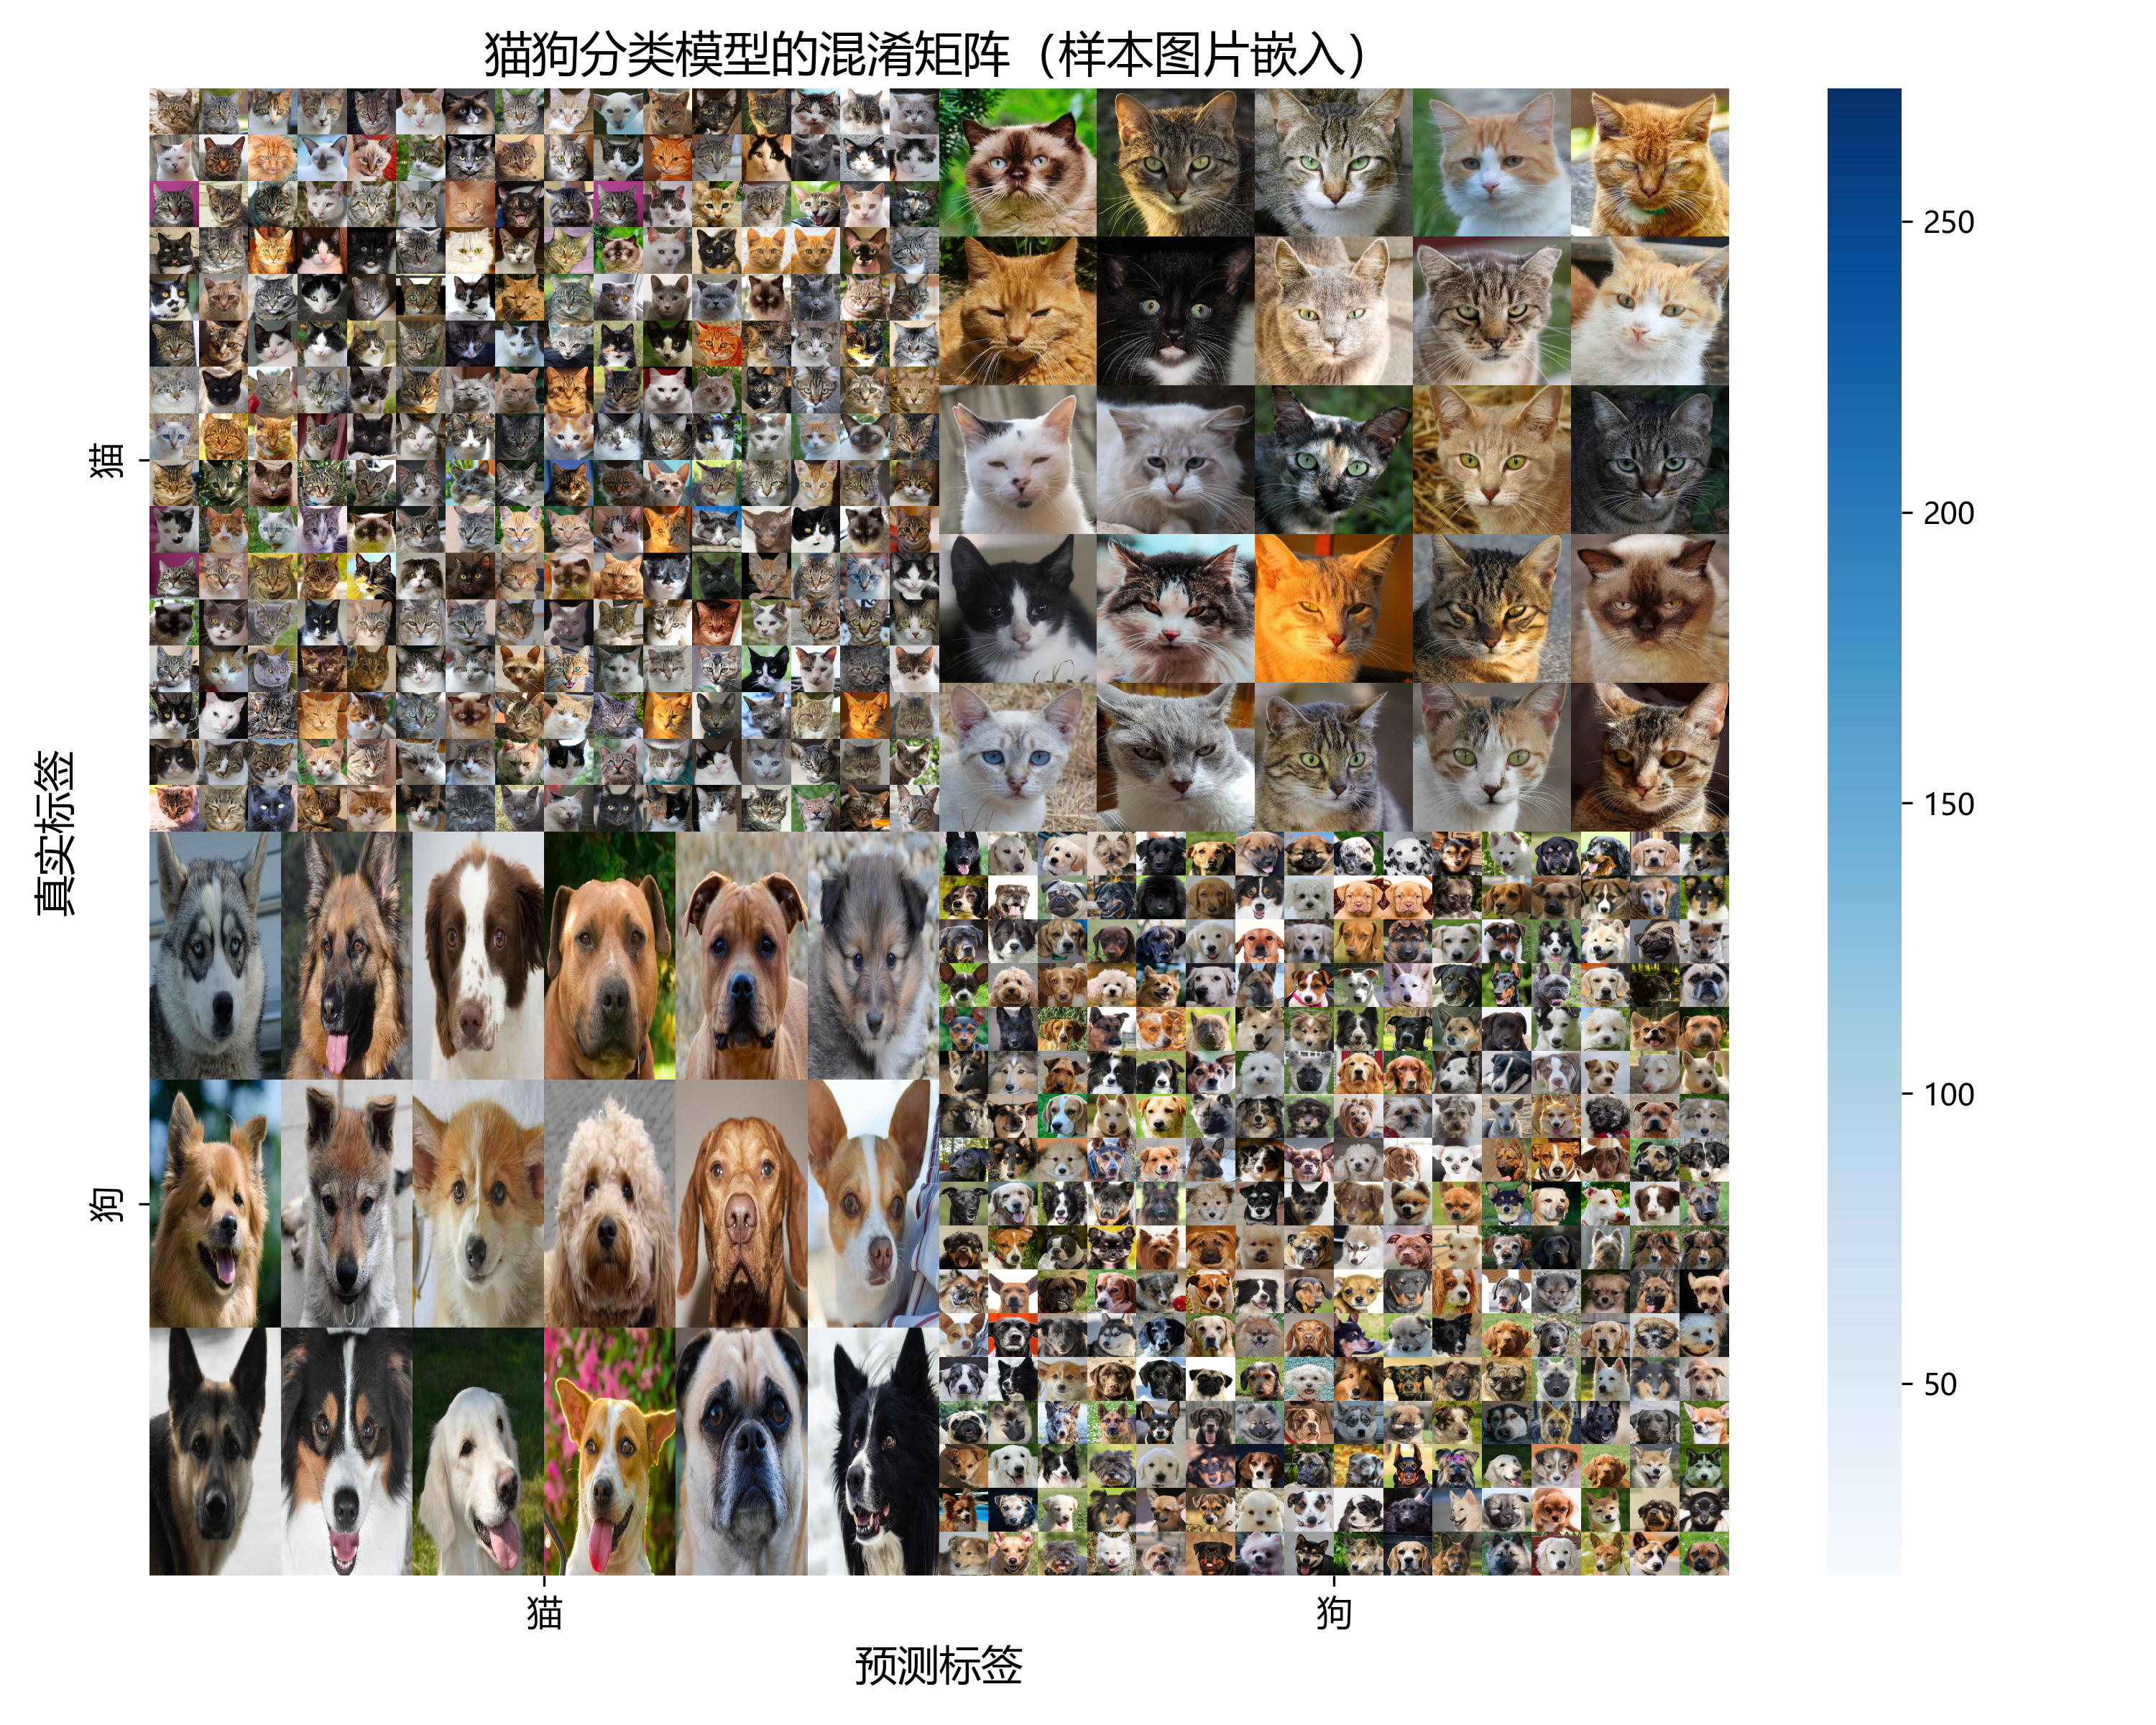
\includegraphics[width=\linewidth]{image/6/confusion_matrix_with_all_images.png}
        \caption{混淆矩阵(图片示例)}
        \label{混淆矩阵(图片示例)}
    \end{subfigure}
    \captionsetup{font=small}  % 调整整体标题的字体大小
    \caption{混淆矩阵展示}
    \label{混淆矩阵展示}
\end{figure}

图~\ref{混淆矩阵展示} (a)展示了模型在测试集上对两种类别(猫和狗)的分类结果。通过统计预测结果与真实标签的交叉关系,混淆矩阵量化了分类模型的性能。左上角格子表示模型正确地将 263 张猫的图片分类为“猫”,右下角格子表示模型正确地将 273 张狗的图片分类为“狗”,说明模型对大部分样本的分类是准确的。右上角格子表示模型错误地将 27 张猫的图片分类为“狗”,而左下角格子表示模型错误地将 18 张狗的图片分类为“猫”,这些非对角线元素反映了分类错误的分布。

根据混淆矩阵的统计结果,猫类的分类准确率为:
\[
\text{猫的准确率} = \frac{263}{263 + 18} \approx 93.6\%
\]
狗类的分类准确率为:
\[
\text{狗的准确率} = \frac{273}{273 + 27} \approx 91.0\%
\]
总体准确率为:
\[
\text{总体准确率} = \frac{263 + 273}{263 + 27 + 273 + 18} \approx 92.3\%
\]

图~\ref{混淆矩阵展示} (b) 在图~\ref{混淆矩阵展示}  (a) 的基础上嵌入了实际样本图片,更直观地展示了分类结果。通过样本图片的直观展示,可以更容易观察到模型分类的错误分布以及正确分类的具体实例。这种可视化方式不仅提升了可读性,还为分析和改进模型性能提供了依据。模型整体表现较好,总体准确率达到 92.3\%,对猫和狗的分类表现接近,但狗的分类误差略高于猫。未来可通过数据增强或调整模型超参数等方法,进一步提升分类性能,尤其是对错误分布更为集中的类别的改进。


\subsection{评估报告}
在生成评估报告时,通常会使用一些常见的评估指标来全面了解模型的表现。这些指标能够分析模型在不同方面的性能,包括它在分类任务中的准确性、可靠性以及综合能力。以下是几个重要的评估指标:

\begin{itemize}
    \item \textbf{精确率 (Precision)}:精确率衡量的是模型预测为某一类别的样本中,实际属于该类别的比例。具体来说,精确率越高,表示模型对于某个类别的预测越准确。
    
    \item \textbf{召回率 (Recall)}:召回率衡量的是实际属于某一类别的样本中,模型成功识别出来的比例。召回率越高,表示模型对该类别的识别能力越强。
    
    \item \textbf{F1 分数 (F1 Score)}:F1 分数是精确率和召回率的调和平均值。它在精确率和召回率之间找到平衡,适用于类别不平衡的情况。F1 分数越高,表示模型在两者之间的表现越好。
    
    \item \textbf{平均损失值 (Average Loss)}:平均损失值是所有测试样本的误差的平均值,表示模型预测结果和真实值之间的差距。较小的损失值意味着模型预测较为准确。
    
    \item \textbf{总体准确率 (Overall Accuracy)}:准确率表示模型预测正确的样本占总样本数的比例。准确率越高,表示模型整体的预测效果越好。
\end{itemize}

\subsubsection{生成分类报告}
为了生成关于分类的报告,使用程序清单~\ref{生成分类报告}生成并打印了每个类别的精确率、召回率和 F1 分数三个方面的信息。
\begin{lstlisting}[language={python},label={生成分类报告},caption={生成分类报告}, basicstyle=\footnotesize\ttfamily, breaklines=true, numbers=left, frame=single,keepspaces=true,showstringspaces=false]
print("分类报告:")
print(classification_report(val_label, val_pre, target_names=train_data.classes))
\end{lstlisting}
\textbf{代码解析:}
\begin{itemize}
    \item \textbf{print(“分类报告:”)}:这行代码输出字符串 “分类报告:”,作为接下来打印分类报告的标题。

    \item \textbf{print(classification\_report(...))}:这行代码调用了\texttt{classification-\\\_report()} 函数来生成并打印模型在验证集上的分类报告。具体来说:
\begin{itemize}
    \item \texttt{val\_label}:包含验证集中所有样本的真实标签。
    \item \texttt{val\_pre}:包含模型对验证集中所有样本的预测结果。
    \item \texttt{target\_names=train\_data.classes}:这部分指定了每个类别的名称,它来自训练数据的类别信息(即猫和狗)。
\end{itemize}
\end{itemize}

\subsubsection{计算总体损失与准确率}
为了从全局视角评估模型的性能,需要对测试集的所有数据进行计算,求出平均损失值和总体准确率。

首先初始化累计变量,代码如程序清单~\ref{初始化累计变量}所示。
\begin{lstlisting}[language={python},label={初始化累计变量},caption={初始化累计变量}, basicstyle=\footnotesize\ttfamily, breaklines=true, numbers=left, frame=single]
running_loss = 0.0
running_corrects = 0
\end{lstlisting}
\textbf{代码解析:}
\begin{itemize}
    \item \textbf{running\_loss = 0.0}:初始化变量 \texttt{running\_loss} 为 0,用于累积每批数据的误差(损失)。该变量将在后续计算中求得所有测试数据的总误差。

    \item \textbf{running\_corrects = 0}:初始化变量 \texttt{running\_corrects} 为 0,用于记录模型正确预测的样本数量。

\end{itemize}

其次遍历测试数据,代码如程序清单~\ref{遍历测试数据}所示。
\begin{lstlisting}[language={python},label={遍历测试数据},caption={遍历测试数据}, basicstyle=\footnotesize\ttfamily, breaklines=true, numbers=left, frame=single]
with torch.no_grad():
    for X, y in test_loader:
        X, y = X.to(device), y.to(device)
        
        outputs = model(X)
        loss = loss_fn(outputs, y)
        _, preds = torch.max(outputs, 1)
        
        running_loss += loss.item() * X.size(0)
        running_corrects += torch.sum(preds == y).item()
\end{lstlisting}
\textbf{代码解析:}
\begin{itemize}
    \item \textbf{with torch.no\_grad()}:此操作禁用梯度计算,用于测试阶段。这样可以减少计算量,加速推理过程,并节省内存。

    \item \textbf{for X, y in test\_loader}:遍历测试数据加载器 \texttt{test\_loader},每次获取一批数据,其中 \texttt{X} 是输入图像,\texttt{y} 是对应的标签。

    \item \textbf{X, y = X.to(device), y.to(device)}:将输入数据 \texttt{X} 和标签     \texttt{y} 移动到指定的计算设备(如 CPU 或 GPU)上,以便进行计算。

    \item \textbf{outputs = model(X)}:将输入图像 \texttt{X} 传入训练好的模型,得到模型的预测结果 \texttt{outputs}。

    \item \textbf{loss = loss\_fn(outputs, y)}:计算模型预测结果 \texttt{outputs} 与实际标签 \texttt{y} 之间的误差(损失)。\texttt{loss\_fn} 是损失函数,用于衡量模型预测的准确性。

    \item \textbf{\_, preds = torch.max(outputs, 1)}:从模型的输出中获取每个样本的预测类别。通过 \texttt{torch.max()} 找到每个样本预测的最大值对应的类别。

    \item \textbf{running\_loss += loss.item() * X.size(0)}:将当前批次的损失值    \texttt{loss.item()} 乘以当前批次的样本数 \texttt{X.size(0)},并累加到\texttt{running\_loss} 中,用于计算总损失。

    \item \textbf{running\_corrects += torch.sum(preds == y).item()}:统计当前批次中预测正确的样本数,并将其累加到 \texttt{running\_corrects} 中。

\end{itemize}

最后进行全局指标的计算,代码如程序清单~\ref{计算全局指标}所示。
\begin{lstlisting}[language={python},label={计算全局指标},caption={计算全局指标}, basicstyle=\footnotesize\ttfamily, breaklines=true, numbers=left, frame=single]
total_loss = running_loss / len(test_loader.dataset)
total_acc  = running_corrects / len(test_loader.dataset)

print(f'\n验证集上的总体损失: {total_loss:.4f}, 准确率: {total_acc:.4f}')
\end{lstlisting}
\textbf{代码解析:}
\begin{itemize}
    \item \textbf{total\_loss = running\_loss / len(test\_loader.dataset)}:计算测试集上的平均损失值,将累积的损失值 \texttt{running\_loss} 除以测试集的样本总数。

    \item \textbf{total\_acc = running\_corrects / len(test\_loader.dataset)}:计算测试集上的总体准确率,将正确预测的样本数 \texttt{running\_corrects} 除以测试集的样本总数。

    \item \textbf{print(f'\textbackslash n验证集上...)}:这一行代码以格式化字符串的方式输出模型在测试集上的平均损失值和总体准确率。“:.4f”表示结果包含保留四位小数的损失值和准确率,方便清晰直观地了解模型在整个测试集上的整体表现。
\end{itemize}

\textbf{输出信息如下:}
\vspace{-2mm} % 在 tcolorbox 下方减小间距
\begin{tcolorbox}[colframe=blue!50!black, colback=blue!10!white, coltitle=black, sharp corners, top=0mm, bottom=0mm, boxrule=0.8mm, breakable, enhanced]
\begin{verbatim}
              precision    recall  f1-score   support

         cat       0.94      0.91      0.92       290
         dog       0.91      0.94      0.92       291

    accuracy                           0.92       581
   macro avg       0.92      0.92      0.92       581
weighted avg       0.92      0.92      0.92       581
\end{verbatim}
\end{tcolorbox}

分类报告中包含了精确率(Precision)、召回率(Recall)、F1 分数(F1-Score)以及支持数量(Support)等重要指标,以下对报告结果进行详细分析:

\begin{itemize}
    \item \textbf{类别“cat”}:
    \begin{itemize}
        \item 精确率(Precision):为 0.94,表示模型将图像分类为“cat”的样本中,94\%是正确的。
        \item 召回率(Recall):为 0.91,表示模型成功识别出所有“cat”样本的 91\%。
        \item F1 分数(F1-Score):为 0.92,是精确率和召回率的调和平均值,反映了模型对“cat”的综合分类表现。
        \item 支持数量(Support):为 290,表示测试集中实际属于“cat”的样本数。
    \end{itemize}
    
    \item \textbf{类别“dog”}:
    \begin{itemize}
        \item 精确率(Precision):为 0.91,表示模型将图像分类为“dog”的样本中,91\%是正确的。
        \item 召回率(Recall):为 0.94,表示模型成功识别出所有“dog”样本的 94\%。
        \item F1 分数(F1-Score):为 0.92,是精确率和召回率的调和平均值,反映了模型对“dog”的综合分类表现。
        \item 支持数量(Support):为 291,表示测试集中实际属于“dog”的样本数。
    \end{itemize}

    \item \textbf{总体准确率(Accuracy)}:
    \begin{itemize}
        \item 模型在测试集上的整体准确率为 0.92,表示测试集中 92\%的样本被正确分类。
    \end{itemize}

    \item \textbf{宏平均(Macro Avg)}:
    \begin{itemize}
        \item 精确率、召回率和 F1 分数分别为 0.92,表示对所有类别的平均表现,不考虑类别样本数量的不均衡。
    \end{itemize}

    \item \textbf{加权平均(Weighted Avg)}:
    \begin{itemize}
        \item 精确率、召回率和 F1 分数分别为 0.92,表示根据各类别样本数量加权后的整体表现,更能反映模型的实际应用效果。
    \end{itemize}
\end{itemize}

从以上报告分析中得出,模型在“cat”和“dog”两个类别上的表现较为均衡,综合指标较高,且整体准确率达到 92\%,说明模型具有良好的分类能力。

\section{总结}

在本章的学习过程中,首先探讨了Python作为人工智能领域编程语言的优势,包括其简洁的语法结构和丰富的社区资源,接着介绍了Python生态系统中不可或缺的几个库——如Pandas、Matplotlib等,对于数据处理、可视化以及模型构建至关重要。随后,继续深入讲解如何运用这些工具进行数据集的准备、数据特征的探索及分析结果的展示,为后续的模型训练做好充分准备。最后通过实际的猫狗识别案例研究展示从数据预处理到使用现代深度学习框架进行模型训练的完整流程。通过猫狗识别项目的构建,逐步动手实践,能够更好地理解和掌握相关人工智能知识,同时积累宝贵的实际操作经验,为进一步探索人工智能领域打下坚实的基础。

\section*{习题}
\begin{enumerate}
    \item \textbf{解释数据预处理的重要性,并描述使用Python如何处理缺失值、异常值等数据质量问题。}\\
    参考答案:数据预处理是机器学习和深度学习中至关重要的步骤,其目的是提高模型的训练效果和预测能力。通过处理缺失值、异常值以及其他数据质量问题,可以确保数据的一致性和可靠性。例如:
    \begin{itemize}
        \item \textbf{缺失值处理}:使用 Python 的 \texttt{pandas} 库可以用均值、中位数或特定值填充缺失值,或者直接删除含有缺失值的样本。
        \item \textbf{异常值处理}:可以通过统计方法(如箱线图分析)识别异常值,并使用替换或删除方法进行处理。
        示例代码:
        \begin{verbatim}
        import pandas as pd
        # 填充缺失值
        df['column'] = df['column'].fillna(df['column'].mean())
        # 删除异常值
        df = df[df['column'] < threshold]
        \end{verbatim}
    \end{itemize}

    \item \textbf{解释学习率的概念及其对训练过程的影响,并举例如果学习率设置不当可能会导致什么问题?}\\
    参考答案:学习率是控制模型在每次迭代时参数更新幅度的超参数。较高的学习率可能使模型在优化过程中震荡或无法收敛,而较低的学习率可能导致收敛速度过慢甚至陷入局部最优。例如:
    \begin{itemize}
        \item \textbf{学习率过高}:模型可能在损失函数中跳跃,无法找到最优解。
        \item \textbf{学习率过低}:模型可能需要更多的训练时间,甚至停留在局部最优。
    \end{itemize}
    动态调整学习率(如使用学习率调度器)是常见的优化策略。

    \item \textbf{在深度学习模型中,隐藏层的数量和神经元个数是如何影响模型的学习能力和复杂度的?}\\
    参考答案:隐藏层的数量和神经元的个数决定了模型的学习能力和复杂度:
    \begin{itemize}
        \item \textbf{隐藏层过少或神经元过少}:模型可能欠拟合,无法捕捉复杂数据的特征。
        \item \textbf{隐藏层过多或神经元过多}:模型可能过拟合,泛化能力较差。
    \end{itemize}
    模型的设计需要在复杂度和性能之间取得平衡。

    \item \textbf{正则化在防止模型过拟合方面起着什么样的作用?}\\
    正则化通过向损失函数中添加约束项,限制模型参数的大小,从而降低模型对训练数据的过度拟合。例如:
    \begin{itemize}
        \item \textbf{L1 正则化}:通过稀疏化参数使模型简单。
        \item \textbf{L2 正则化}:通过惩罚参数的平方值降低参数复杂度。
        \item \textbf{Dropout}:通过随机忽略部分神经元,减少过拟合。
    \end{itemize}

    \item \textbf{为什么在模型训练中要将数据集划分为训练集和测试集?两者之间的比例分配对模型性能评估有何影响?}\\
    参考答案:数据集划分为训练集和测试集是为了评估模型的泛化能力:
    \begin{itemize}
        \item \textbf{训练集}:用于调整模型参数。
        \item \textbf{测试集}:用于评估模型的性能。
    \end{itemize}
    通常,训练集和测试集的比例分配为 80:20 或 70:30。测试集过小可能导致评估不准确,而测试集过大会减少训练样本,影响模型性能。

    \item \textbf{在批次处理中什么是批量大小(batch\_size),它对模型训练的影响是什么?请举例说明在不同的应用场景下如何选择合适的批量大小。}\\
    参考答案:批量大小是每次迭代中用于计算梯度的样本数。批量大小的选择影响模型的收敛速度和稳定性:
    \begin{itemize}
        \item \textbf{小批量}(如 32 或 64):计算资源需求小,适合小型数据集。
        \item \textbf{大批量}(如 256 或 512):训练速度快,但对显存需求较高。
    \end{itemize}
    示例场景:
    \begin{itemize}
        \item 小型数据集:选择较小的批量大小(如 32)。
        \item 大型数据集:选择较大的批量大小(如 256)。
    \end{itemize}

    \item \textbf{在执行模型训练时,为什么要记录每轮训练的损失值和准确率?}\\
    参考答案:记录每轮训练的损失值和准确率可以:
    \begin{itemize}
        \item 帮助监控模型的训练过程。
        \item 识别潜在问题,例如过拟合或欠拟合。
        \item 判断模型是否收敛或需要调整超参数。
    \end{itemize}

    \item \textbf{损失函数在机器学习中的目的是什么?}\\
    参考答案:损失函数是衡量模型预测值与真实值之间差距的标准,目的是指导模型优化参数,使预测值更接近真实值。例如,回归问题中常用的均方误差(MSE),分类问题中常用的交叉熵损失。

    \item \textbf{可视化在数据分析和模型理解中的作用?}\\
    参考答案:可视化能够直观展示数据的分布、模型的学习情况和预测结果,有助于:
    \begin{itemize}
        \item 发现数据中存在的异常或趋势。
        \item 理解模型训练过程中的变化(如损失曲线)。
        \item 对比不同模型的性能。
    \end{itemize}
\end{enumerate}

% \begin{enumerate}
%     \item 解释数据预处理的重要性,并描述使用Python如何处理缺失值、异常值等数据质量问题。
%     \item 解释学习率的概念及其对训练过程的影响,并举例如果学习率设置不当可能会导致什么问题?
%     \item 在深度学习模型中,隐藏层(的数量和神经元个数是如何影响模型的学习能力和复杂度的?
%     \item 正则化在防止模型过拟合方面起着什么样的作用?
%     \item 为什么在模型训练中要将数据集划分为训练集和测试集?两者之间的比例分配对模型性能评估有何影响?
%     \item 什么是批量大小,它对模型训练的影响是什么?请举例说明在不同的应用场景下如何选择合适的批量大小。
%     \item 在执行模型训练时,为什么要记录每轮训练的损失值和准确率?
%     \item 损失函数在机器学习中的目的是什么?
%     \item 可视化在数据分析和模型理解中的作用?
% \end{enumerate}

